%% main_ppgco_ufu.tex v1.0, Lásaro Camargos e Denise Guliato
% adaptado de modeloABNT2.tex, v1.0 athila 
% ------------------------------------------------------------------------
% ------------------------------------------------------------------------
% eesc: Modelo de Trabalho Acadêmico (tese de doutorado, dissertação de
% mestrado e trabalhos monográficos em geral) em conformidade com 
% ABNT NBR 14724:2011. Esta classe estende as funcionalidades da classe
% abnTeX2 elaborada de forma a adequar os parâmetros exigidos pelas 
% normas USP e do departamento de elétrica da Escola de Engenharia 
% de São Carlos - USP.
% ------------------------------------------------------------------------
% ------------------------------------------------------------------------

% ------------------------------------------------------------------------
% Opções:
% 	tesedr:     Formata documento para tese de doutorado
%	qualidr:    Formata documento para qualificação de doutorado
% 	dissertmst: Formata documento para dissertação de mestrado
% 	qualimst:   Formata documento para qualificação de mestrado
% ------------------------------------------------------------------------
\documentclass[dissertmst]{ppgco}
%Não altere o comando seguinte. O título de seu trabalho será especificado mais adiante.
\title{Análise térmica de canais de Poiseuille: Comparação de abordagem semi analítica com numérica (MFSim) e DNS}

% ---
% PACOTES
% ---

% ---
% Pacotes fundamentais 
% ---
\usepackage{cmap}				% Mapear caracteres especiais no PDF
\usepackage{lmodern}				% Usa a fonte Latin Modern			
\usepackage{makeidx}            	% Cria o indice
\usepackage{hyperref}  			% Controla a formação do índice
\usepackage{lastpage}			% Usado pela Ficha catalográfica
\usepackage{indentfirst}			% Indenta o primeiro parágrafo de cada seção.
\usepackage{nomencl} 			% Lista de simbolos
\usepackage{graphicx}			% Inclusão de gráficos
\usepackage{amsmath}
\usepackage{wrapfig}
% ---

% ---
% Pacotes adicionais, usados apenas no âmbito do Modelo eesc
% ---
\usepackage{lipsum}				       % para geração de dummy text
\usepackage[printonlyused]{acronym}
\usepackage[table]{xcolor}
% ---


% ---
% Informações de dados para CAPA e FOLHA DE ROSTO
% ---
%
% Título:
%	1. Título em português
%	2. Título em inglês
\titulo{Análise térmica de canais de Poiseuille: Comparação de abordagem semi analítica com numérica (MFSim) e DNS}{Análise térmica de canais de Poiseuille: Comparação de abordagem semi analítica com numérica (MFSim) e DNS}
%
% Autor:
%	1. Nome completo do autor
%	2. Formato de nome para bibliografia
\autor{Felipe José Oliveira Ribeiro}{Ribeiro, Felipe}
%
% Cidade
\local{Uberlândia}
% Ano de defesa
\data{2022}
% Área de concentração da pesquisa
\areaconcentracao{Engenharia Aeronáutica}
% Nome do orientador
\orientador{Aristeu da Silveira Neto}
% ---

% ---
% compila o indice
% ---
\makeindex
% ---

% ---
% Compila a lista de abreviaturas e siglas
% ---
\makenomenclature
% ---

% ---
% Inserir ficha catalográfica
%
% Caso o comando \inserirfichacatalografica seja definido, a %ficha catalográfica
% será inserida atrás da folha de rosto. Caso contrário a página será deixada em
% branco.
%
% CUIDADO: Esta opção deve ser preenchida antes do comando \maketitle
% ---
%entre em contato com a biblioteca para obter a sua ficha catalográfica em arquivo pdf. Essa %folha só será inserida no documento após a sua defesa.

\inserirfichacatalografica{fichaCatalografica.pdf}
% ---

% ---
% Inserir folha de aprovação
%
% Caso o comando \inserirfolhaaprovacao seja definido, a a folha de aprovação
% será inserida. Além disso, conforme Resolução CoPGr 5890, as informações 
% de rodapé são inseridas apropriadamente na folha de rosto.
%
% CUIDADO: Esta opção deve ser preenchida antes do comando \maketitle
% ---
% baseie-se no modelo desse documento e gere a sua folha de %rosto em arquivo pdf.

\inserirfolhaaprovacao{folhaAprovacao.pdf}
% ---

% ----
% Início do documento
% ----

\begin{document}

% ----------------------------------------------------------
% ELEMENTOS PRÉ-TEXTUAIS
% ----------------------------------------------------------
\pretextual

% ---
% Insere Capa, Folha de rosto, Ficha catalográfica (se inserida)
% e folha de aprovação (se inserida).
% ---
\maketitle

% ---

% ---
% Agradecimentos
% ---
\imprimiragradecimentos{
Agradeço, a cima de tudo, à minha família, por me apoiar por todos esses anos e nunca medir esforços ao ajudar minha trajetória acadêmica e profissional. Agradeço também aos grandes mestres que tive, em especial, ao professo Aristeu da Silveira Neto, por me guiar por muitos anos em um caminho de aprendizado e evolução. Também é oportuno agradecer a todas as instituições envolvidas nos trabalhos de pesquisa que pavimentaram o caminho até este trabalho. O laboratório de mecânica dos fluidos (MFLab) da Faculdade de Engenharia Mecânica (FEMEC) da Universidade Federal de Uberlândia (UFU). PETROBRAS, CNPq, CAPES e FAPEMIG que contribuíram financeiramente com trabalhos acadêmicos de grande importância na minha trajetória. Finalmente agradeço aos meus colegas, ao amor da minha vida e à todas as pessoas queridas que sempre trazem alegria e conforto para os meus dias.
}
% ---
% ---
% RESUMO e ABSTRACT
% ---

% Resumo em português - as palavras entre chaves são as palavras-chave do trbalho
\begin{resumo}{mecânica dos fluidos, CFD, ensino de engenharia, métodos numéricos, equações de Navier Stokes, turbulência}

No presente trabalho o autor desenvolve uma abordagem semi-exata para análise térmica em escoamentos turbulentos de Poiseuille. Parametriza-se o modelo com base nos métodos descritos em \cite{felipe1}, em seguida, compara-se os resultados com os de métodos numéricos advindos do MFSim e DNS. O modelo físico consistiu em um canal entre placas planas infinitas de fluxo térmico constante que variam linearmente de temperatura no sentido da corrente, resultando em um regime estatisticamente permanente para os perfis de temperatura e velocidade. A parametrização do número de Prandtl turbulento e da constante de Cebeci foram modificadas visando a obtenção de melhor acurácia quando comparada com a solução em DNS. Os resultados foram validados com simulações no MFSim e casos simulados via DNS, constatando-se forte concordância.

\end{resumo}

% Resumo em inglês
\begin{abstract}{Turbulent Prandtl number, Cebeci's constant, Turbulent Poiseuille flow, Genetic algorithm, DNS.}

In the present paper the author develops a semi-exact approach for thermal analysis in turbulent Poiseuille flows. The model is parameterized based on the methods described in \cite{felipe1}, then the results are compared with the numerical methods derived from MFSim and DNS. The physical model consisted of a channel between two infinite flat plates of constant heat flux that vary linearly in temperature in the streamwise direction, resulting in a statistically steady regime for the temperature and velocity profiles. The parameterization of the turbulent Prandtl number and the Cebeci constant were modified in order to obtain better accuracy when compared to the DNS solution. The results were validated with simulations in MFSim and cases simulated via DNS, showing strong agreement.

\end{abstract}
% ---

% ---
% inserir lista de ilustrações
% ---
\listailustracoes
% ---

% ---
% inserir lista de tabelas
% ---
\listatabelas
% ---
% ---
% inserir o sumario
% ---
\sumario
% ---

% ----------------------------------------------------------
% ELEMENTOS TEXTUAIS
% ----------------------------------------------------------
\mainmatter

% ----------------------------------------------------------
% Introdução
% ----------------------------------------------------------
\chapter{Introdução}

\noindent 

	A simulação computacional é uma ferramenta de emprego crescente, que não se limita ao domínio da engenharia, sendo ampliada para aplicações em diversos setores da ciência contemporânea. Já é possível modelar simulações para campos aerodinâmicos, biológicos, meteorológicos e até financeiros. Tal recurso é extremamente útil para a compreensão de fenômenos complexos, de variadas amplitudes no domínio temporal e para a economia de recursos e tempo em projetos de engenharia.
	
	A engenharia moderna possui como alguns dos principais desafios a otimização de sistemas já existentes e a modelagem de novos sistemas com excelentes rendimentos mecânico e térmico. Ainda, essas melhorias devem ocorrer em paralelo com um baixo custo associado de forma a manter a competitividade no mercado. Antes do avanço tecnológico das últimas décadas, a resolução de problemas físicos demandava um grande esforço e custo em função da necessidade de reprodução material, mas esse método pôde ser substituido com teorias bem trabalhadas e fundamentadas em experimentações passadas, modelagens físicas e matemáticas aplicadas em uma resolução numérica-computacional.
	
	Dentre os vários ramos da engenharia, a mecânica dos fluidos é um grande exemplo de aplicação dos métodos supracitados. Tópicos como turbulência, troca de calor e interação fluido-estrutura são trabalhados de forma extensiva na pesquisa, e têm apresentado resultados muito coerentes com aqueles observados pelo método empírico. 
	
	Este trabalho objetiva a execução de análises matemáticas e discretizações numéricas para os transportes por difusão e advecção para os casos unidimensional e bidimensional, sob a metodologia explícita e implícita. Tais mecanismos são observados na transferência de energia térmica em escoamentos laminares, de transição e turbulentos em proporções particulares para cada caso. Os diferentes tratamentos do termo temporal são trabalhados de forma conjunta para a comparação da relação entre custo computacional e estabilidade numérica de ambos. A partir da modelagem numérica das equações associadas, se produz um código, ou modelo computacional, que resolve numericamente o problema a partir de uma condição inicial e condições de contorno conhecidas, finalmente comparando a solução numérica com a analítica.
	
	%Por fim, escoamentos heterogêneos, também tratados neste trabalho, são de grande importância para a mecânica dos fluidos devido à sua extensa ocorrência na prática da engenharia mecânica. O estudo de tais escoamentos possibilita uma modelagem de carregamento de particulado com o fluido durante a extração de petróleo ou a troca de calor em um líquido em transição de fase, por exemplo.
	
\newpage
	

 \section{Metodologia}
 % --------------------------------------------------------------------------

\noindent

	A metodologia proposta para o presente trabalho de iniciação científica se baseia
na definição de problemas, estudando primeiramente os casos particulares, e uma vez
compreendida a natureza do conteúdo, seguindo para problemas mais gerais e complexos.

	Inicialmente verifica-se na literatura as dinâmicas envolvidas nos mecanismos propostos para este estudo. A partir das relações obtidas nessa revisão, elabora-se uma discretização a partir de métodos numéricos e realiza-se a implementação dos mesmos em um código computacional. As rotinas são confeccionadas na linguagem de programação Fortran, para familiarização do aluno com a linguagem base dos códigos do Laboratório de Mecânica dos Fluidos Computacional (MFLab) da Faculdade de Engenharia Mecânica (FEMEC) da Universidade Federal de Uberlândia.
 

\subsection{Difusão}

\noindent

	A difusão é um mecanismo de transporte que possui diferentes definições nos campos da química, biologia e física. Especificamente para o caso de transferência de calor, a difusão é bem definida matematicamente por uma equação diferencial parcial (EDP), que envolve uma derivada parcial de primeira ordem no domínio temporal e uma derivada parcial de segunda ordem no domínio espacial. Os termos são relacionados, através de uma constante (difusividade), à um termo fonte, resultante da diferença desses elementos, como indicado na Eq. (\ref{Difusaoone}).
	
\begin{align}
 \label{Difusaoone}
 f(x,y,z,t) = \dfrac{\partial \phi}{\partial t} - \alpha \nabla^2 \phi
\end{align}

	Assim, para o caso unidimensional, obtém-se a relação dada pela Eq.(\ref{Difuni}).
	
\begin{align}
 \label{Difuni}
 f(x,t) = \dfrac{\partial \phi}{\partial t} - \alpha \left(\dfrac{\partial^2 \phi}{\partial x^2}\right)
\end{align}

	E para o caso bidimensional, obtém-se a relação dada pela Eq.(\ref{Difbi}).
	
\begin{align}
 \label{Difbi}
 f(x,y,t) = \dfrac{\partial \phi}{\partial t} - \alpha \left[ \left(\dfrac{\partial^2 \phi}{\partial x^2}\right) - \left(\dfrac{\partial^2 \phi}{\partial y^2}\right)\right]
\end{align}
	
	A difusividade ($\alpha$) é traduzida fisicamente como a rapidez com que a energia térmica é transportada espacialmente para dado material. O termo fonte ($f$), por sua vez, se traduz na resultante da diferença das parciais, que deve ser nulo para a solução da difusão. 

\subsection{Advecção}

\noindent

	A advecção é um mecanismo de transporte que também é presente em vários campos de estudo, dado pela transferência de calor juntamente com a transferência de espécie. Esse fenômeno é modelado matemáticamente pela Eq. (\ref{Adveccao}).
	
\begin{align}
\label{Adveccao}
f(x,y,z,t) = \dfrac{\partial \phi}{\partial t} + c \nabla \phi
\end{align}

	Para o caso unidimensional, de forma análoga ao caso da difusão, tem-se que a relação fica como indicada pela Eq. (\ref{advuni}).
	
\begin{align}
\label{advuni}
f(x,t) = \dfrac{\partial \phi}{\partial t} + c \dfrac{\partial \phi}{\partial x}
\end{align}

	Para o caso bidimensional, obtém-se a relação dada pela Eq. (\ref{advbi}).
	
\begin{align}
\label{advbi}
f(x,t) = \dfrac{\partial \phi}{\partial t} + cx \dfrac{\partial \phi}{\partial x} + cy \dfrac{\partial \phi}{\partial y}
\end{align}
	
	A velocidade ($c$) é traduzida fisicamente como a velocidade com que a variação térmica ocorre com a movimentação de massa na direção avaliada, sendo que essa velocidade pode ser positiva ou negativa. Já o termo fonte ($f$), se traduz na resultante da soma das parciais, que deve ser nulo para a solução da difusão.

\subsection{Difusão e Advecção}
\noindent

	O efeito combinado dos dois mecanismos é obtido de forma intuitiva através da soma dos termos difusivos e advectivos. Pode-se então descrever o fenômeno através da Eq.(\ref{difadv}).
	
\begin{align}
\label{difadv}
f(x,y,z,t) = \dfrac{\partial \phi}{\partial t} - \alpha \nabla^2 \phi + c \nabla \phi
\end{align}

	Novamente, para o caso unidimensional, simplesmente exclui-se dois termos espaciais, resultando na Eq.(\ref{difaduni}).

\begin{align}
\label{difaduni}
f(x,t) = \dfrac{\partial \phi}{\partial t} - \alpha \left(\dfrac{\partial^2 \phi}{\partial x^2}\right) + c \dfrac{\partial \phi}{\partial x}
\end{align}	

	Finalmente, para o caso bidimensional, exclui-se apenas um termo espacial, resultando na Eq.(\ref{difadbi}).

\begin{align}
\label{difadbi}
f(x,t) = \dfrac{\partial \phi}{\partial t} - \alpha \left[ \left(\dfrac{\partial^2 \phi}{\partial x^2}\right) + \left(\dfrac{\partial^2 \phi}{\partial y^2}\right)\right] + cx \dfrac{\partial \phi}{\partial x} + cy \dfrac{\partial \phi}{\partial y}
\end{align}	
	
\subsection{Malha}
\noindent

	Para este trabalho a malha é não adaptativa, devido ao baixo custo operacional das rotinas. Então, faz-se uso da condição de Courant-Friedrichs-Lewy (CFL) para a confecção da mesma.
	
	A CFL é uma condição necessária para a solução de certas equações diferenciais parciais pelo método de diferenças finitas. Tal condição é obtida de uma análise do diferencial de tempo explícito em relação ao diferencial espacial. Como conclusão, percebe-se que proporções maiores que aquelas ditadas pelo CFL correspondente resultam em sistemas instáveis e não convergentes.
	
	Para o caso da difusão, o passo temporal se relaciona ao passo espacial como indicado pela Eq.(\ref{Cflone}) para o caso unidimensional, e pela Eq.(\ref{Cfltwo}) para o caso bidimensional.
	
\begin{align}
\label{Cflone}
\Delta t = CFL \dfrac{(\Delta x)^2}{\alpha}
\end{align}

\begin{align}
\label{Cfltwo}
\Delta t = min \left(CFL \dfrac{(\Delta x)^2}{\alpha} , CFL \dfrac{(\Delta y)^2}{\alpha}\right)
\end{align}

	Para o caso da advecção, o passo temporal se relaciona ao passo espacial como indicado pela Eq.(\ref{Cflthree}) para o caso unidimensional, e pela Eq.(\ref{Cflfour}) para o caso bidimensional.
	
\begin{align}
\label{Cflthree}
\Delta t = CFL \dfrac{\Delta x}{\mid c \mid}
\end{align}

\begin{align}
\label{Cflfour}
\Delta t = min \left(CFL \dfrac{\Delta x}{\mid cx \mid}, CFL \dfrac{\Delta y}{\mid cy \mid}\right)
\end{align}

	Ainda, para os efeitos conjulgados, os passos temporal e espacial se relacionam como indicado pela Eq.(\ref{Cflfive}) para o caso unidimensional e como indicado pela Eq.(\ref{Cflsix}) para o caso bidimensional.
	
\begin{align}
\label{Cflfive}
\Delta t = min \left(CFL \dfrac{(\Delta x)^2}{\alpha}, CFL \dfrac{\Delta x}{\mid c \mid}\right)
\end{align}

\begin{align}
\label{Cflsix}
\Delta t = min \left(CFL \dfrac{(\Delta x)^2}{\alpha} , CFL \dfrac{(\Delta y)^2}{\alpha}, CFL \dfrac{\Delta x}{\mid cx \mid}, CFL \dfrac{\Delta y}{\mid cy \mid}\right)
\end{align}

	A malha para este trabalho é composta de células de dimensões $\Delta x$ por $\Delta y$, nucleadas em seu centro. A coordenada utilizada para as operações são referentes aos núcleos. 
	
Para um dado domínio em uma direção qualquer, sabe-se que as condições de contorno devem ser aplicadas nas arestas da célula. Para que isso ocorra, pode-se trabalhar na suposição de uma célula fantasma, que aplicada no método numérico gera a condição de contorno na parede, ou simplesmente usar a metade de uma célula para o contorno do domínio. A modelagem matemática numérica para os problemas aqui propostos é baseada na segunda condição. Assim, as células possuem dimensões fracionadas na fronteira.
	Uma representação de uma malha não adaptativa de duas dimensões é ilustrada a seguir na Figura(1.1).
\newline
\newline	

\begin{figure}[ht!]
	\label{malhim}
	\centering
	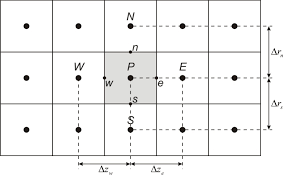
\includegraphics[width=60mm]{Imagens/malha.png}
	\caption{Exemplo de uma malha não adaptativa}
\end{figure}


% ----------------------------------------------------------
% Fundamentação
% ----------------------------------------------------------
\chapter[Fundamentação Teórica]{Fundamentação Teórica}


\section{Modelo físico}

Neste trabalho, procura-se analisar o perfil térmico sobre um escoamento turbulento no canal de Poiseuille. Ele pode ser definido como um escoamento confinado entre duas placas infinitas. Nelas, o escoamento atinge velocidade igual a zero (condição de não deslizamento) e estão em regime de fluxo térmico constante. Tais placas encontram-se perpendiculares ao eixo $y$. O eixo $z$ é definido como auto-similar tanto na velocidade quanto na temperatura, resultando em um domínio plano (Fig.\ref{descricaoGeometrica}). O escoamento foi considerado incompressível e o fluido foi considerado newtoniano. Neste sistema físico, o fluido escoa, em média, somente na direção do eixo $x$.
Os números de Reynolds ($Re = \frac{2R \overline{U}}{\nu}$) variam de $4560$ a $41441$, resultando em um regime turbulento.

\begin{figure}[h!]
	\centering
	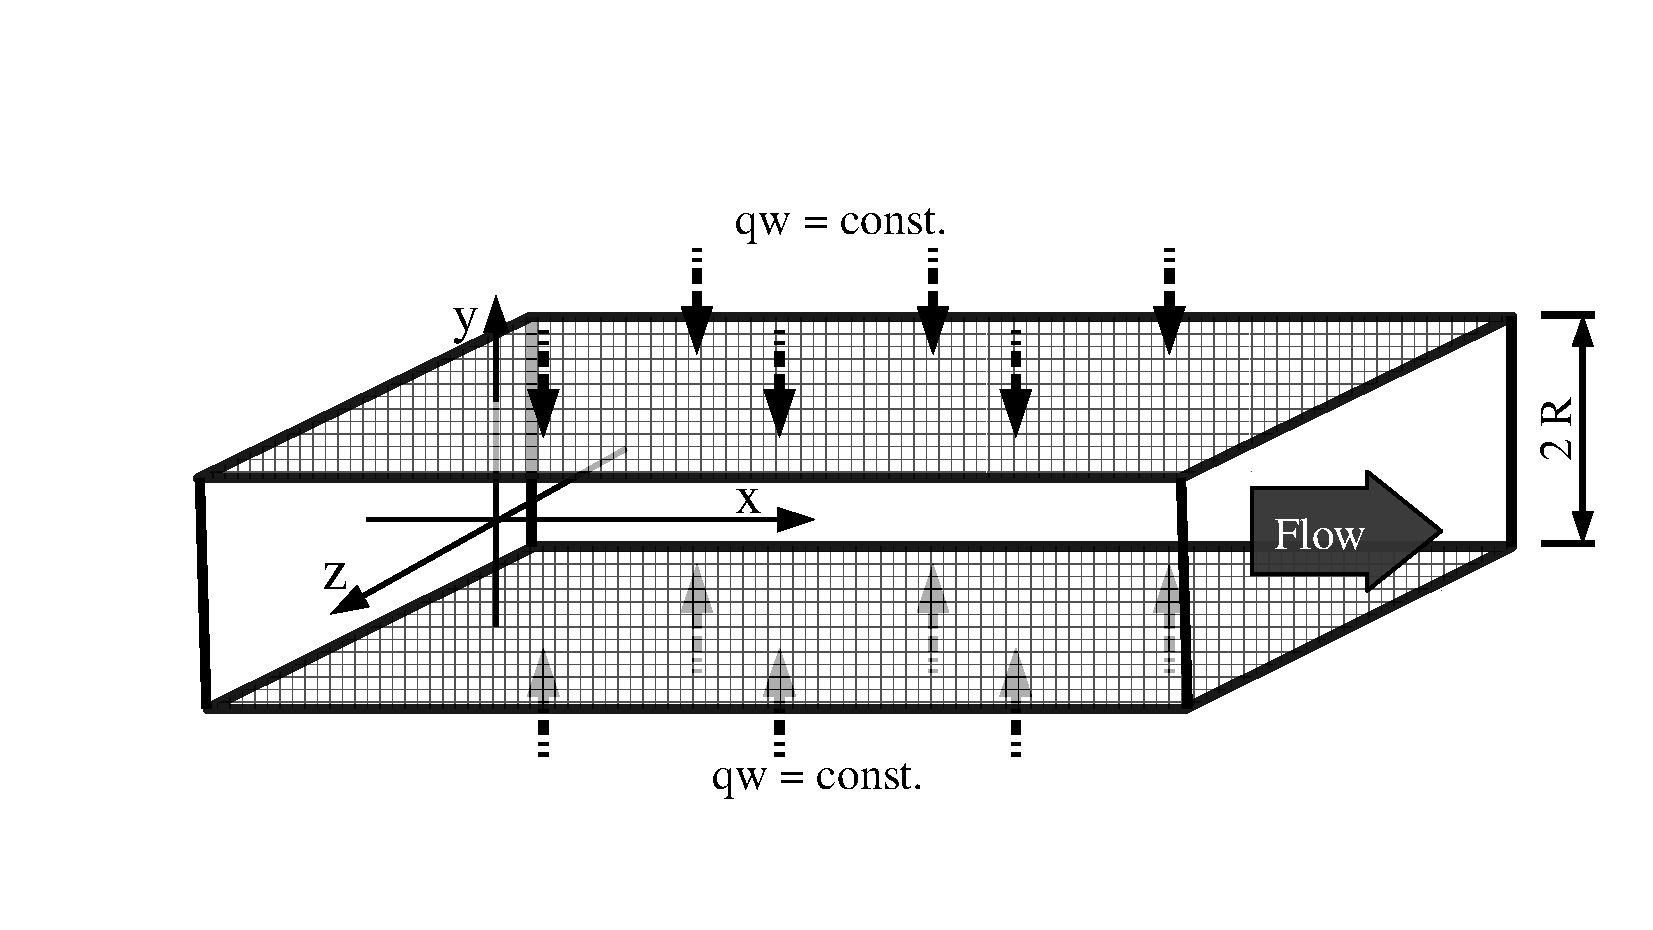
\includegraphics[angle=0, trim={0mm 23mm 0mm 35mm}, clip , scale=0.42]{cap_fundamentacao/canal1.pdf}
	\caption{Definição geométrica e condições de contorno.}
  \legend{Fonte: Autor.}
	\label{descricaoGeometrica}
\end{figure}

Estas foram as suposições efetuadas para o problema proposto, que serão consideradas no modelo matemático diferencial adiante.

\section{Modelo matemático diferencial}
A formulação matemática do problema foi baseada nas equações de continuidade, de Navier-Stokes \cite{Cengel}, e na equação de transporte de energia térmica \cite{Incropera}: 

\begin{equation}
  \frac{\partial u}{\partial t} + \frac{\partial u^2}{\partial x} + \frac{\partial uv}{\partial y} + \frac{\partial uw}{\partial z} = - \frac{1}{\rho} \frac{\partial {p}}{\partial x} + \nu \left( \frac{\partial^2 u}{\partial x^2} + \frac{\partial^2 u}{\partial y^2} + \frac{\partial^2 u}{\partial z^2}   \right)
\end{equation}

\begin{equation}
  \frac{\partial \rho}{\partial t} +  \frac{\partial (\rho u)}{\partial x} + \frac{\partial (\rho v)}{\partial y} + \frac{\partial (\rho w)}{\partial z} = 0
\end{equation}

\begin{equation}
  \frac{\partial T}{\partial t} + {\frac{\partial{}}{\partial{x}} (uT)} + {\frac{\partial{}}{\partial{y}} (vT)} + {\frac{\partial{}}{\partial{z}} (wT)}
  =
  {\frac{\partial{}}{\partial{x}}} \left(\alpha {\frac{\partial{T}}{\partial{x}}} \right) +
  {\frac{\partial{}}{\partial{y}}} \left(\alpha {\frac{\partial{T}}{\partial{y}}} \right) +
  {\frac{\partial{}}{\partial{z}}} \left(\alpha {\frac{\partial{T}}{\partial{z}}} \right)
\end{equation}

\begin{equation}\label{resfriamentoDeNewton}
  q_{conv.} = \dot{m} C_p \Delta T_m.
\end{equation}

Eq.\ref{resfriamentoDeNewton} é baseada na lêi de resfriamento de newton \cite{Incropera}, onde $\dot{m}$ é a vazão volumétrica, $C_p$ é a capacidade calorífica específica, $\Delta T_m$ é a diferença de temperatura entre a superfície e o fluido, e $q_{conv.}$ é a taxa de transferência de calor por convecção.

\subsection{O estudo dos comportamentos médios}
Para simplificar o sistema, foi realizado um tratamento estatístico nas equações. Cada grandeza foi dividida entre valor médio e flutuações, sendo que a média torna-se independente do tempo:

\begin{equation}
  \overline{f}({x})=\frac{1}{t_f - t_i} \int_{t_i}^{t_f} f({x} , t) dt.
\end{equation}

\begin{equation}
  f({x} , t) = \overline{f}({x}) + f^\prime ({x} ,t),
\end{equation}

também é possível realizar as seguintes operações com as flutuações:

\begin{equation}
  \begin{cases}
  \overline{f^\prime ({x} ,t)} = 0 , & \quad   \\
  \overline{\overline{f({x})}} = \overline{f({x})} , & \quad   \\
  \overline{f^\prime ({x} ,t)\overline{f({x})}} = 0 ,& \quad   \\
  \overline{f^\prime ({x} ,t)g^\prime ({x} ,t)} \neq 0 , & \quad   \\
  \overline{  \overline{g({x})} \ \overline{f({x})}  } = {\overline{g({x})}} \ {\overline{f({x})}} , & \quad   \\
  \end{cases}
\end{equation}

A partir destas operações foi possível simplificar o sistema de equações. É possível se representar geométricamente também essa separação entre a média e flutuação na Figura \ref{figura.1}:

\begin{figure}[h!]
	\centering
	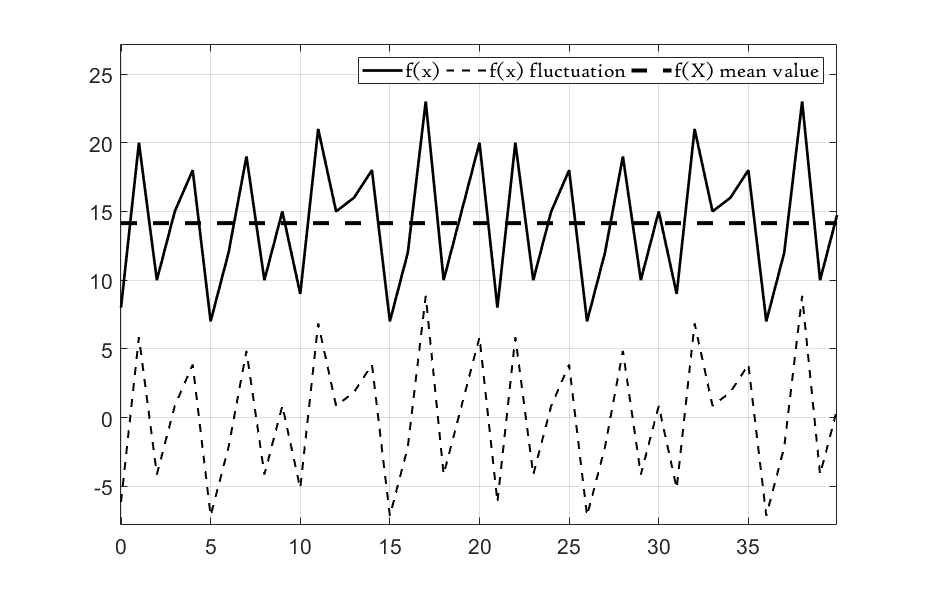
\includegraphics[angle=0, scale=0.60]{medios}
	\caption{Representação geométrica da separação entre os valores médios e as flutuações.}
  \legend{Fonte: Autor.}
	\label{figura.1}
\end{figure}

Dessa forma, aplicando as simplificações, obtêm-se as equações médias da continuidade (Eq.\ref{mass}), de Navier-Stokes (Eq.\ref{dynamics}) e de balanço de energia (Eq.\ref{energy permanent}):

\begin{equation}\label{mass}
\frac{\partial \overline{u}}{\partial x} = 0,
\end{equation}

\begin{equation}\label{dynamics}
\frac{\partial \overline{u} \, \overline{v}}{\partial y} = 
- \frac{1}{\rho} \frac{\partial \overline{p}}{\partial x} + \frac{\partial}{\partial y}\left(\nu \frac{\partial \overline{u}}{\partial y} - \overline{u^\prime v^\prime}\right),
\end{equation}


\begin{equation}\label{energy permanent}
\frac{\partial{}}{\partial{x}} \left(\overline{T^\prime u^\prime}\right) + \frac{\partial{}}{\partial{x}}\left(\overline{u} \overline{T}\right)     + 
\frac{\partial{}}{\partial{y}} \left(\overline{T^\prime v^\prime}\right) + \frac{\partial{}}{\partial{y}}\left(\overline{v} \overline{T}\right) 
=
{\frac{\partial{}}{\partial{x}}} \left(\alpha {\frac{\partial{\overline{T}}}{\partial{x}}} \right) +
{\frac{\partial{}}{\partial{y}}} \left(\alpha {\frac{\partial{\overline{T}}}{\partial{y}}} \right). 
\end{equation}

Sendo $\overline{u}$ e $\overline{v}$ as velocidades médias e $u^\prime$ e $v^\prime$ as flutuações na velocidade nos eixos $x$ e $y$, $\rho$ a massa específica, $\overline{p}$ a pressão média, $\nu$ a viscosidade cinemática, $\overline{T}$ a temperatura média, $T^\prime$ a flutuação na temperatura e $\alpha$ a difusividade térmica.

O método, independente da variável do tempo e baseado em comportamentos médios, é caracterizado como um exemplo de metodologia RANS (Reynolds-averaged Navier-Stokes).


\subsection{O regime permanente térmico}

O campo de velocidade média atinge regime estatisticamente permanente no canal (Fig. \ref{figure.3}), mas o mesmo não ocorre para o campo de temperatura, pois um fluxo térmico constante é imposto sobre as paredes. A temperatura continua aumentando no domínio, nunca se estabilizando.
Outra diferença entre os dois domínios é o fato de que o perfil de velocidade mantém-se constante no sentido do fluxo. Isso possibilita que o sistema seja representado unidimensionalmente, simplificando drasticamente as formulações matemáticas. O mesmo não pode ser dito para o campo de temperatura média, as temperaturas aumentam linearmente no sentido do fluxo (Fig. \ref{figure.2}):

\begin{figure}[h!]
	\centering
	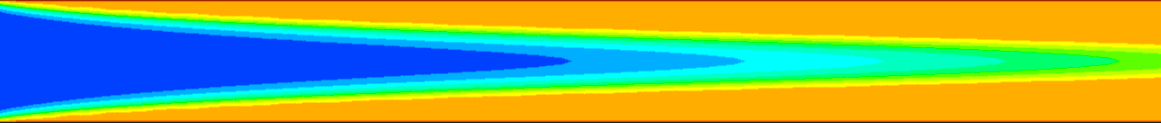
\includegraphics[angle=0, scale=0.4]{cap_fundamentacao/temperatura.png}
	\caption{Campo de temperatura média no canal de Poiseuille. O perfil de temperatura no canal aumenta linearmente na direção do fluxo.}
  \legend{Fonte: Autor, em simulação realizada no Mfsim.}
	\label{figure.2}
\end{figure}
\begin{figure}[h!]
	\centering
	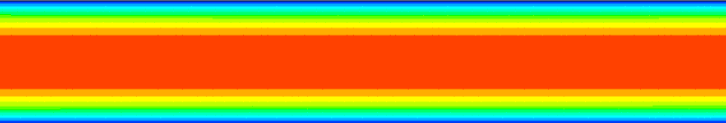
\includegraphics[angle=0, height=1.35cm , width=12.3cm]{cap_fundamentacao/velocidade.png}
	\caption{Campo de velocidade média no canal de Poiseuille. O perfil se mantém constante na direção do fluxo.}
  \legend{Fonte: Autor, em simulação realizada em código próprio.}
	\label{figure.3}
\end{figure}

Para simplificar o equacionamento do campo de temperatura médio, um balanço de energia térmica foi estudado (Eq. \ref{c_h_e}):

\begin{equation}\label{c_h_e}
q_{conv.} = \dot{m} C_p \Delta T_m,
\end{equation}

A partir da equação de balanço de energia térmica, pode-se obter a temperatura média no domínio:

\begin{equation}
2q_w b \Delta x = \dot{m} C_p \Delta T_m,
\end{equation}\\

\begin{equation}
\Delta T_m = \frac{2q_w b \Delta x}{\dot{m} C_p},
\end{equation}

Onde $q_w$ é o fluxo de calor nas paredes, $b$ é a largura do canal e $\Delta x$ é a distância entre as paredes.\\
Então, subistituindo $ \dot{m} = u_m 2R b \rho $ onde $u_m$ é a velocidade média no domínio, $R$ é o raio do canal e $\rho$ é a massa específica, e se assumindo que $ \Delta T_m = \frac{\partial{\left(\overline{T}_m\right)}}{\partial{x}} \Delta x $: 

\begin{equation}\label{c_h_ee}
\frac{\partial{\left(\overline{T}_m\right)}}{\partial{x}} = \frac{q_w}{u_m R \rho C_p}.
\end{equation}

Como todos os termos à direita da equação são constantes, a temperatura média varia linearmente no sentido da corrente.\\
Para melhor entender a temperatura nas paredes, uma formulação de convecção termal foi estudada:

\begin{equation}
q_w = h A \left( T_w(x) - \overline{T}_m(x)\right).
\end{equation}

Como se tem um fluxo completamente desenvolvido, pode-se afirmar que o valor de $h$ é constante. Assim, usando-se a Eq. \ref{c_h_ee}, é possível se concluir que:

\begin{equation}
\frac{d T_w(x)}{d x} = \frac{d \overline{T}_m(x)}{d x} = Cte.
\end{equation}	

Dessa forma, considerando que a temperatura nas paredes varia linearmente, assim como a temperatura média, é possível se extender esse gradiente no domínio completo ao se considerar as condições de contorno e a simetria do systema. Assim, nas paredes é imposto um gradiente de temperatura constante, criando-se um regime de condição de contorno de fluxo térmico constante. Consequentemente, todo o campo de temperatura varia linearmente na direção da corrente e com o tempo.
O valor de temperatura foi então decomposto no seguinte modo:

\begin{equation}
   T^\ast(y) = T(x,y) - T_w(x),
\end{equation}


 Onde $T^\ast(y)$ é a temperatura relativa, $T(x,y)$ é a temperatura absoluta e $T_w(x)$ é a temperatura na parede.\\

 Assim, analisando-se $T^\ast(Y)$, vemos auto-similaridade no sentido da corrente, resultando em um equacionamento unidimentional representativo com solução em $T^\ast(y)$.

 Finalmente Eq. \ref{energy permanent}:

\begin{equation}
\begin{split}
\frac{\partial{}}{\partial{x}} \left(\overline{(T^\ast + T_w)^\prime} \overline{ u^\prime}\right) + \frac{\partial{}}{\partial{x}}\left(\overline{(T^\ast + T_w)} \overline{u}\right)+ 
\frac{\partial{}}{\partial{y}} \left(\overline{(T^\ast + T_w)^\prime} \overline{ v^\prime}\right) + \frac{\partial{}}{\partial{y}}\left(\overline{(T^\ast + T_w)} \overline{v}\right) = \\
{\frac{\partial{}}{\partial{x}}} \left(\alpha {\frac{\partial{\overline{(T^\ast + T_w)}}}{\partial{x}}} \right) +
{\frac{\partial{}}{\partial{y}}} \left(\alpha {\frac{\partial{\overline{(T^\ast + T_w)}}}{\partial{y}}} \right). 
\end{split}
\end{equation}

Então a expressão pode ser desenvolvida ainda mais algebricamente considerando todas as velocidades médias nas direções $y$ e $z$ nulas:

\begin{equation}\label{equation_var}
{\frac{\partial{}}{\partial{y}}} \left(\alpha {\frac{\partial{\overline{T^\ast}}}{\partial{y}}}   
- \left(\overline{ T^{\ast\prime} v^\prime}\right) \right)
= 
\overline{u}\frac{\partial{\overline{T_w}}}{\partial{x}}.
\end{equation}

\subsection{A hipótese de Bousinesq}

A hipótese de Bousinesq é uma aproximação que permite a análise de sistemas de convecção térmica em regime permanente. No caso do presente trabalho a hipótese foi empregada no termo $\overline{T^{\ast\prime}  v^\prime}$, que pode, então, ser modelado como segue:

\begin{equation}\label{bou}
-\left(\overline{ T^{\ast\prime}  v^\prime}\right) = 
\alpha_t \frac{\partial{\overline{T^\ast}}}{\partial{y}}.
\end{equation}

Onde $\alpha_t$ é a difusividade térmica turbulenta do fluido. Assim, substituindo-se Eq. \ref{bou} na Eq. \ref{equation_var}:

\begin{equation}\label{oiiiii}
{\frac{\partial{}}{\partial{y}}} \left[(\alpha + \alpha_t)  \frac{\partial \overline{T^\ast}}{\partial y} \right]
= 
\overline{u}\frac{\partial{\overline{T_w}}}{\partial{x}}. 
\end{equation}

\subsection{O comprimento de mistura de Prandtl}

O termo da difusão térmica turbulenta, $\alpha_t$, precisa ser modelado. Para modelá-lo, usou-se o conceito clássico do número de prandtl turbulento que é:

\begin{equation}
Pr_t = \frac{\nu_t}{\alpha_t}.
\end{equation} 

A viscosidade cinemática turbulenta $\nu_t$ precisa ser modelada. O valor do número de prandtl turbulento pode ser definido como $Pr_t = 0.71$, como consta na literatura.

Com o modelo de comprimento de mistura de Prandtl, é definido:

\begin{equation}
\nu_t = {l^2_m} \left| \frac{\partial \overline{u}}{\partial y} \right|.
\end{equation}

\begin{equation}\label{3332x}
\alpha_t = \frac{{l^2_m}}{Pr_t} \left| \frac{\partial \overline{u}}{\partial y} \right|.
\end{equation}

Onde $l_m$ é o comprimento de mistura. Então substituindo-se Eq. \ref{3332x} na Eq. \ref{oiiiii}:

\begin{equation}\label{equationquasela}
{\frac{\partial{}}{\partial{y}}} \left( \left( \alpha   
+ \frac{{l^2_m} \left| \frac{\partial \overline{u}}{\partial y} \right|}{Pr_t} \right) \frac{\partial \overline{T^\ast}}{\partial y} \right)
= 
\overline{u}\frac{\partial{}}{\partial{x}}\left(\overline{T_w}\right)  .
\end{equation}

É possível notar, quando se analisa a dinâmica do fluido, que para valores positivos de $y$, a derivada da velocidade é sempre negativa, com uma velocidade que decresce com y. Resultando em:

\begin{equation}
{\frac{\partial{}}{\partial{y}}} \left( \left( \alpha   
- \frac{{l^2_m}}{Pr_t}\frac{\partial \overline{u}}{\partial y} \right) \frac{\partial \overline{T^\ast}}{\partial y} \right)
= 
\overline{u}\frac{\partial{}}{\partial{x}}\left(\overline{T_w}\right)  .
\end{equation}

\subsection{O comprimento de mistura}

O comprimento de mistura $ l_m $ precisa ser modelado. Os estudos experimentais de nikuradse foram usados para modelar esse parâmetro para escoamentos de canal, como segue:

\begin{equation}
L\left(\frac{y}{R}\right) = \frac{l_m}{R} = 0.14 - 0.08 \left(\frac{y}{R}\right)^2 - 0.06\left(\frac{y}{R}\right)^4.
\end{equation}

Para maior completude do modelo, cebeci e bradshaw adicionaram a função de amortecimento de Van Driest:

\begin{equation}\label{eqution_mixturelength}
L\left(\frac{y}{R}\right)  = \frac{l_m}{R} = \left\{ 0.14 - 0.08 \left(\frac{y}{R}\right)^2 - 0.06\left(\frac{y}{R}\right)^4\right\}\left\{  1 - e^{[(\frac{y}{R} - 1) \frac{Re_\tau}{A}]}\right\},
\end{equation}

Com $A = 26$ como a constante de Cebeci. Assim, tem-se o comprimento de mistura definido como:

\begin{equation}
l_m = L R,
\end{equation}

Sendo $L$ uma função no eixo $y$, dado pela equação \ref{eqution_mixturelength}. Então a equação \ref{equationquasela} pode ser escrita da seguinte forma:

\begin{equation}\label{cebeciconstant}
{\frac{\partial{}}{\partial{y}}} \left( \left( \alpha   
- \frac{{L}^2 R ^2}{Pr_t}\frac{\partial \overline{u}}{\partial y} \right) \frac{\partial \overline{T^\ast}}{\partial y} \right)
= 
\overline{u}\frac{\partial{}\left(\overline{T_w}\right)  }{\partial{x}}.
\end{equation}

Usando-se coordenadas de parede, a equação foi adimensionalizada, para que pudesse ser comparada com a literatura. As considerações adotadas foram: $ \tilde{y} = \frac{y . Re_\tau}{R} $, $ \tilde{\overline{u}} = \frac{\overline{u}}{u_\tau} $ , $ \tilde{\overline{T}} = \frac{\overline{T}}{T_\tau} $ , $ \tilde{\overline{T^\ast}} = \frac{\overline{T^\ast}}{T_\tau} $ , $Re_\tau = \frac{u_\tau R}{\nu}$, $Pr_t = \frac{\nu_t}{\alpha_t}$, $Pr = \frac{\nu}{\alpha}$, $T_\tau = \frac{q_w}{\rho C_p u_\tau}$, $\frac{\partial{\left(T_m\right)}}{\partial{x}} = \frac{q_w}{u_m  R \rho  C_p } $ e $\frac{\partial \overline{p}}{\partial x} = - \frac{u_\tau^2 \rho}{R} $. Que, ao se substituir em (\ref{cebeciconstant}) resultou em (\ref{equationultima}):
\\
\begin{equation}\label{equationultima}
{\frac{\partial{}}{\partial{\tilde{y}}}} \left( \left( \frac{Re_\tau}{Pr}   
- \frac{{L}^2 Re_\tau ^3}{Pr_t}\frac{\partial \tilde{\overline{u}}}{\partial \tilde{y}} \right) \frac{\partial \tilde{\overline{T^\ast}}}{\partial \tilde{y}} \right)
= 
\frac{\tilde{\overline{u}}}{\tilde{u_m}}.
\end{equation}

É importante observar que existe a velocidade na equação (\ref{equationultima}), ou seja, para o desenvolvimento do problema térmico é necessário o desenvolvimento do perfil dinâmico do canal. Para isso, foi utilizada uma metodologia rans previamente estabelecida \cite{luigi}, conforme segue:

\begin{equation}\label{finalequationvelocity}	
\frac{\partial \tilde{\overline{u}}}{\partial \tilde{y}} = - \frac{2 \tilde{y} \frac{1}{Re_\tau} }{ 1 + \sqrt{ 1 + 4 L ^2 Re_\tau ^2 \tilde{y}}}.
\end{equation}	

Assim, tem-se a primeira derivada da velocidade determinada algebricamente.

\newpage

\section{Modelo matemático numérico}

Para discretizar a equação diferencial, um domínio euleriano foi declarado. Para a velocidade foi aplicado um método runge-kutta de quarta ordem, enquanto a temperatura foi arranjada em um esquema de diferenças centradas que teve que ser resolvido implicitamente.
O modelo dinâmico é resolvido primeiro, e seu resultado é usado na solução do perfil térmico. O centro da célula foi usado de forma que a parede fosse colocada no centro da célula e um ponto entre as células fosse colocado no ponto central do canal. A convergência dos resultados numéricos é mostrada na figura \ref{sistema}:

\begin{figure}[!h]
	\centering
	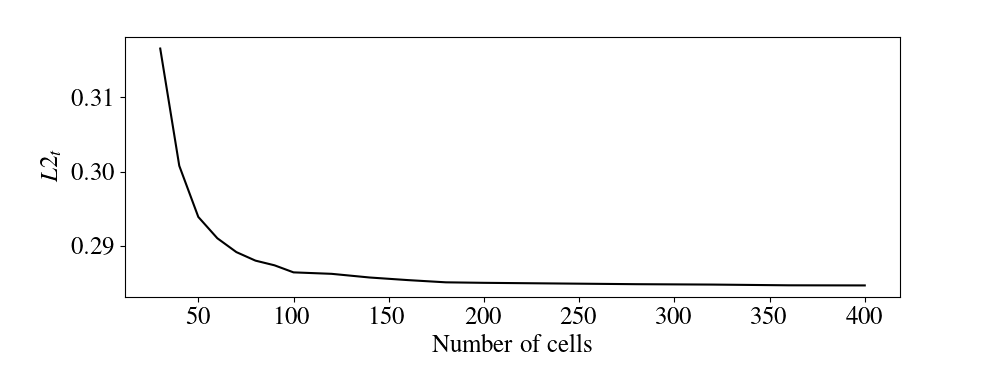
\includegraphics[angle=0, trim={10mm 0mm 0mm 0mm}, clip , scale=0.50]{fotos_formatacao_final/Convergence}
	\caption{Norma L2 de simulação térmica comparado a dns até 400 células, com $Re_\tau = 1020$.}
	\label{sistema}
\end{figure}

Quanto maior o número de elementos na malha, maior a acurácia do resultado até atingida a convergência quando comparado aos resultados em DNS. A partir disso, os erros observados deixam de ser devido ao método numérico e têm significância quanto aos ajustes aplicados, como, por exemplo, a hipótese de bousinesq.

Dessa forma, para cada resultado, deu-se um número suficiente de elementos para que houvesse a convergência do erro numérico.


\chapter{Ajustes propostos}

\subsection{Resultados via método canônico}
Inicialmente o número de prandtl turbulento, $Pr_t = 0,71$, foi usado como na literatura. Os resultados obtidos apresentados na figura \ref{figuraresultados1} são comparados com os dns de \cite{dns1020} e \cite{dns150}, com a norma l2.\\

\begin{figure}[!h]
  \centering
  \begin{minipage}{0.49\textwidth}
    \centering
    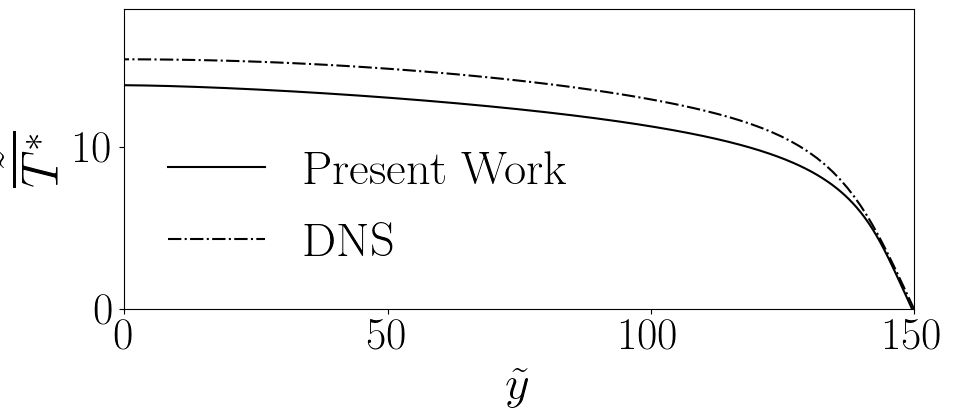
\includegraphics[angle=0, scale=0.32]{fotos_formatacao_final/Temperature_150_071_classico}
    \subcaption{$Re_\tau = 150$, $L2_t = 1.42$}
  \end{minipage}
  \hfill
  \begin{minipage}{0.49\textwidth}
    \centering
    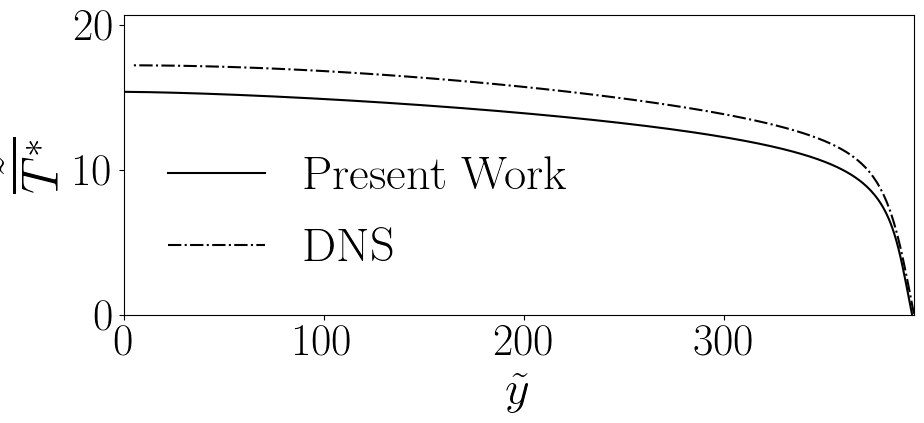
\includegraphics[angle=0, scale=0.32]{fotos_formatacao_final/Temperature_395_071_classico}
    \subcaption{$Re_\tau = 395$, $L2_t = 1.55$}
  \end{minipage}
  \begin{minipage}{0.49\textwidth}
    \centering
    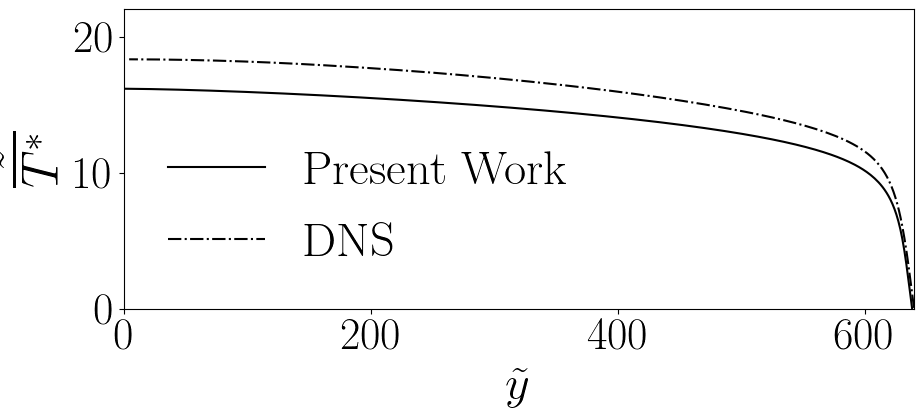
\includegraphics[angle=0, scale=0.32]{fotos_formatacao_final/Temperature_640_071_classico}
    \subcaption{$Re_\tau = 640$, $L2_t = 1.79$}
  \end{minipage}
  \hfill
  \begin{minipage}{0.49\textwidth}
    \centering
    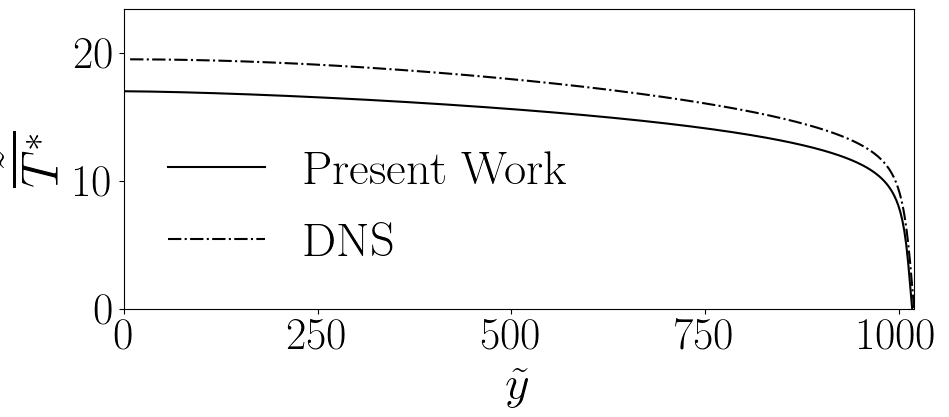
\includegraphics[angle=0, scale=0.32]{fotos_formatacao_final/Temperature_1000_071_classico}
    \subcaption{$Re_\tau = 1020$, $L2_t = 2.04$}
  \end{minipage}
  \caption{Distribuição de temperatura para $Pr_t = 0.71$, $A = 26$ e $Pr = 0.71$.} 
  \label{figuraresultados1}
\end{figure}

Os primeiros resultados mostram um forte efeito negativo das aproximações empregadas. Percebeu-se que o número de prandtl turbulento teve grande influência no resultado.
A grandeza podia ser encontrada no banco de dados do DNS, e observou-se que ela variava em função da distância da parede (\cite{dns1020} e \cite{dns150}) (figure \ref{figure5}).
O valor então foi extraído do banco de dados e usado como parâmetro durante uma simulação do método descrito no presente trabalho, obtendo-se uma norma L2 de $ 0,19 $ para $ Re_t = 640 $.

Assim foi validado que o problema estava na parametrização do número de prandtl turbulento.

\begin{figure*}[h!]
	\centering
	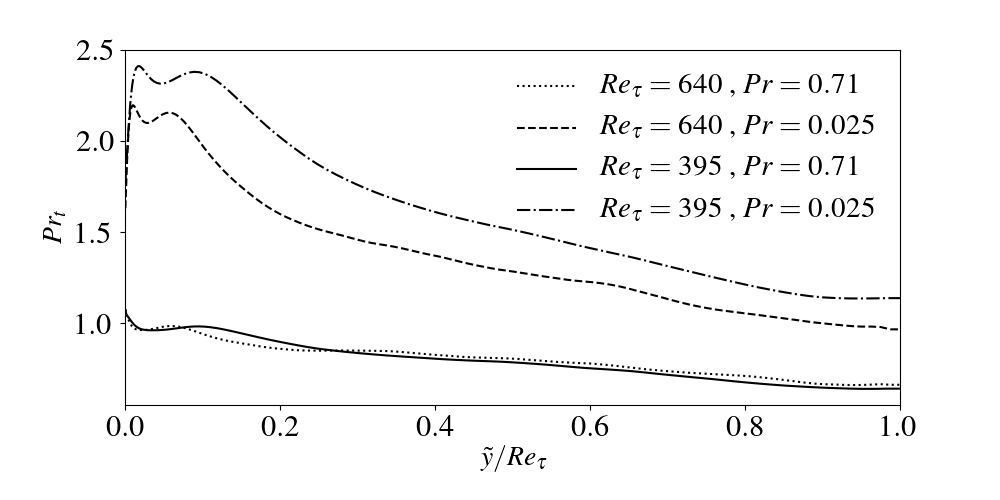
\includegraphics[angle=0, scale=0.62]{fotos_formatacao_final/DNS_PRt}
	\caption{Número de Prandtl turbulento adquirido do DNS em função de $ \tilde{y}/Re_\tau $, a distância até a parede no canal.}
	\label{figure5}
\end{figure*}

Assim, iniciou-se o esforço de propor uma parametrização ajustada para o número de prandtl turbulento. Neste sentido tentou-se ajustar um valor para que o erro fosse mínimo, quando comparado com o DNS. Neste sentido, aplicou-se a metodologia de algoritmos baseados em evolução diferencial \cite{Price2013}.

\subsection{O meta modelo adquirido via evolução Diferencial (DE)}

Foi utilizado um algoritmo de evolução diferencial \cite{diferential} na procura da melhor parametrização possível do Prandtl turbulento. Neste algorítmo, arbitra-se um valor editável pelo algorítmo e uma função objetiva cujo programa tentará minimizar ajustando valores na variável editável. Durante as iterações de simulações, os resultados direcionam o algorítmo, cujas tentativas concentram-se mais e mais ao redor do mínimo encontrado pela função objetiva.

Considerou-se o número de prandtl turbulento como variável livre e a norma L2 como função objetiva.
O erro foi calculado comparando a temperatura resultante com os dados DNS (\cite{dns1020} e \cite{dns150}). Obteve-se um número prandtl turbulento de $ 0.9$, para o número de Reynolds $ Re_\tau = 1020$.

É importante ressaltar que o número de prandtl turbulento foi encontrado como uma constante. Apesar de, nos dados do DNS ele ser apresentado como um vetor de valores em função da distância da parede, optou-se por buscar uma constante representativa, de forma a se simplificar a abordagem.



Pode-se ver adiante a forma como o algorítmo genético evoluiu para encontrar o valor de $ Pr_t $ ideal, ou seja, o valor que resultada no menor erro.

\begin{figure}[!h]
	\centering
	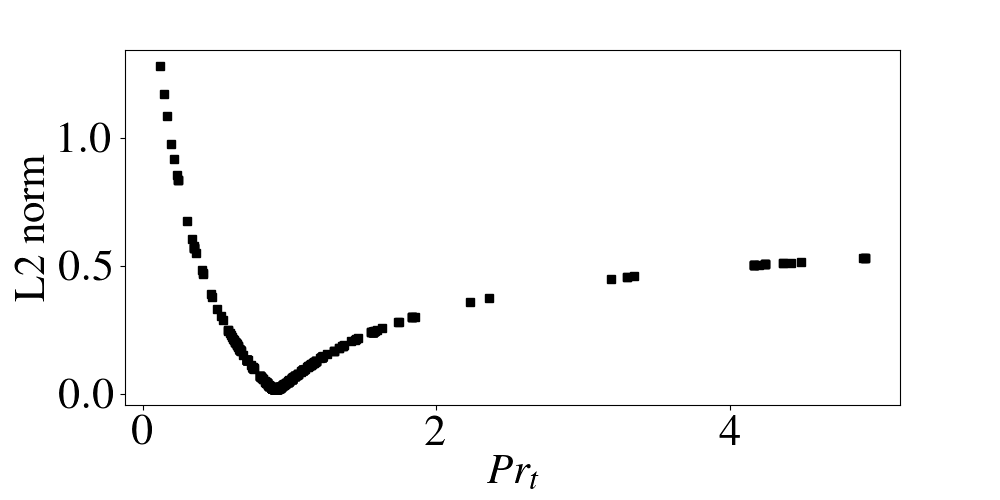
\includegraphics[angle=0, scale=0.61]{fotos_formatacao_final/Genetic_amostra}
	\caption{Iterações de algoritmo genético, com simulações para $Re_\tau = 1020$. Convergência em $Pr_t = 0.9 $.}
\end{figure}

O número de prandtl turbulento obtido, $Pr_t = 0.9$ que minimiza o erro no campo da temperatura, foi considerado aos demais números de Reynolds, resultando na figura \ref{primeiros}.

\begin{figure*}[!h]
	\centering
	\begin{minipage}[t]{0.5\textwidth}
		\centering
		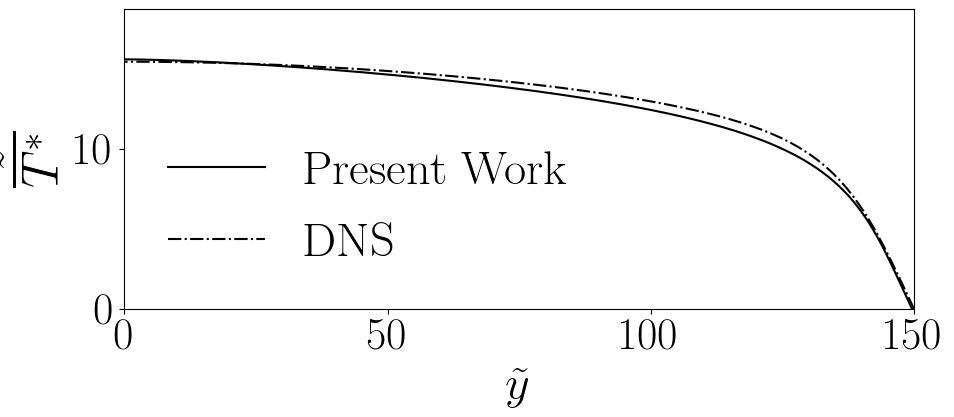
\includegraphics[angle=0, scale=0.34]{fotos_formatacao_final/Temperature_150_071_Prt0905_A26}
		\subcaption{$Re_\tau = 150$, $L2_t = 0.34$}
	\end{minipage}
	\begin{minipage}[t]{0.45\textwidth}
		\centering
		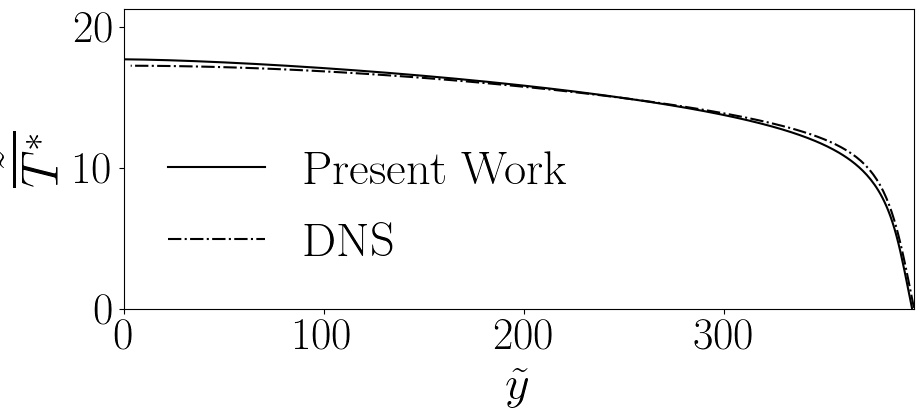
\includegraphics[angle=0, scale=0.34]{fotos_formatacao_final/Temperature_395_071_Prt0905_A26}
		\subcaption{$Re_\tau = 395$, $L2_t = 0.23$}
	\end{minipage}
	\begin{minipage}[t]{0.5\textwidth}
		\centering
		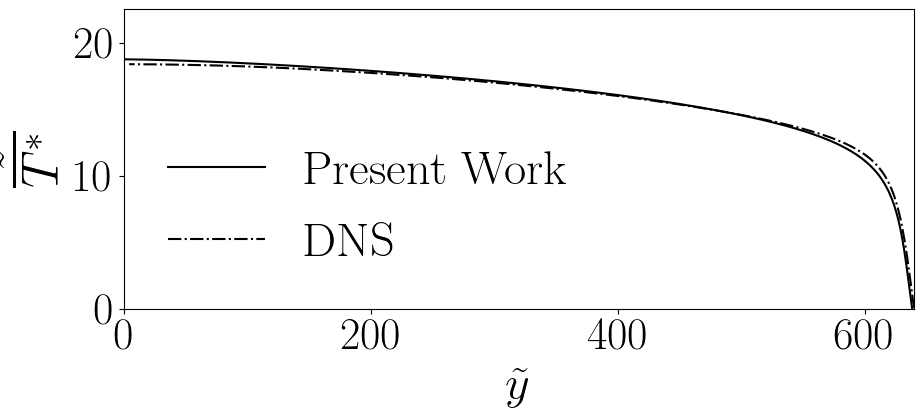
\includegraphics[angle=0, scale=0.34]{fotos_formatacao_final/Temperature_640_071_Prt0905_A26}
		\subcaption{$Re_\tau = 640$, $L2_t = 0.19$}
	\end{minipage}
	\begin{minipage}[t]{0.45\textwidth}
		\centering
		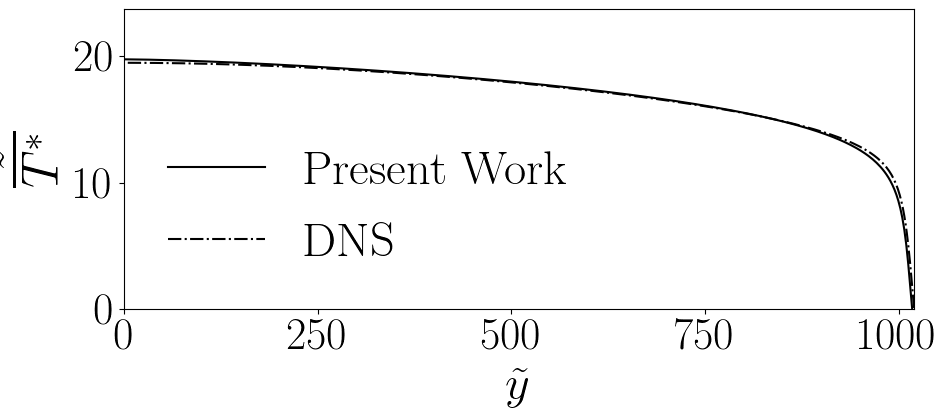
\includegraphics[angle=0, scale=0.34]{fotos_formatacao_final/Temperature_1000_071_Prt0905_A26}
		\subcaption{$Re_\tau = 1020$, $L2_t = 0.14$}
	\end{minipage}	
	\caption{Perfis de temperatura para simulações com $Pr_t = 0.9 $, $A = 26$ e $Pr =0.71$ }
	\label{primeiros}
\end{figure*}

Apesar de os resultados serem melhores, se comparados aos da figura \ref{figuraresultados1}, ainda havia mais espaço para melhoras. O número de Prandtl turbulento varia com o número de Reynolds turbulento, como pode ser visto em fig.\ref{figure5}, então um modelo que leve em conta a grandeza estaria mais próximo do correto. 
Para se obter a curva de $Pr_t$ em função do $Re_\tau$, o mesmo algorítmo foi usado, obtendo-se um valor de número de Prandtl turbulento ideal para cada número de Reynolds turbulento disponível resultados de DNS (\cite{dns1020} and \cite{dns150}).

Os valores obtidos podem ser conferidos na tabela \ref{tabela1}:

\begin{table}[!h]
	\centering
	\caption{Números de prandtl turbulentos ideais ajustados para cada número de Reynolds turbulento, com a constante de cebeci $A = 26$.}
	\begin{tabular}{ll}
		  \hline
		  $Re_\tau$ & $Pr_t$\\
		  \hline
		  150  &   0.94531\\
		  395  &   0.89531\\
		  640  &   0.89531\\
		  1020 &   0.90000\\ 
		  \hline
	\end{tabular}
	\label{tabela1}
\end{table}

Realizando um ajuste de curva polinomial, um modelo ajustado para o número de prandtl turbulento em função do número de reynolds foi desenvolvido:

\begin{equation}
  \begin{split}
    Pr_t = -4.5604 * 10^{-10} Re_\tau^3 + 9.5690 * 10^{-7} Re_\tau^2 - 6.1715 *10 ^{-4} Re_\tau + 1.0178 .
  \end{split}
\end{equation}

Os resultados das simulações foram muito acurados, ainda mais do que as simulações com os números turbulentos de prandtl definidos como valores médios dos dados dns (fig.\ref{figure5}). Estes resultados podem ser observados na figura \ref{figura_9}:

\begin{figure*}[!h]
	\centering
	\begin{minipage}[t]{0.5\textwidth}
		\centering
		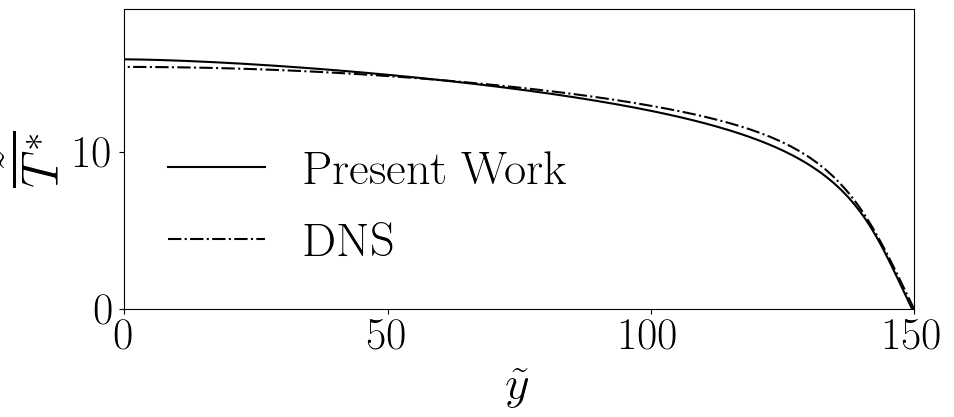
\includegraphics[angle=0, scale=0.34]{fotos_formatacao_final/Temperature_150_071_Prt(Ret)_A26}
		\subcaption{$Re_\tau = 150$, $L2_t = 0.26$}
	\end{minipage}
	\begin{minipage}[t]{0.45\textwidth}
		\centering
		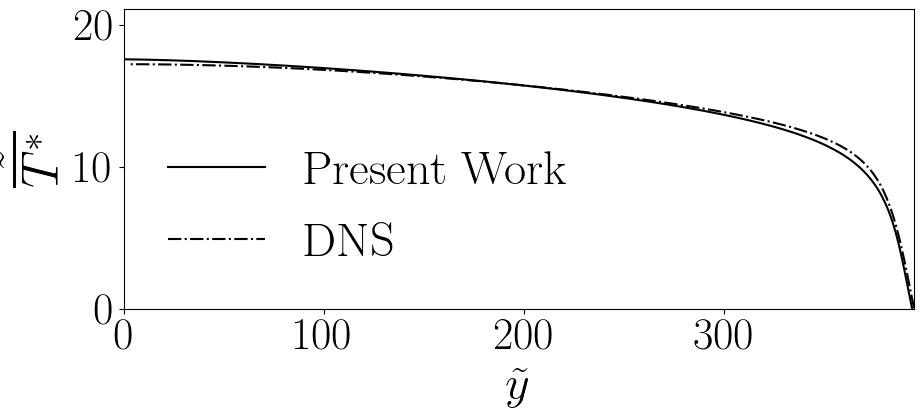
\includegraphics[angle=0, scale=0.34]{fotos_formatacao_final/Temperature_395_071_Prt(Ret)_A26}
		\subcaption{$Re_\tau = 395$, $L2_t = 0.22$}
	\end{minipage}
	\begin{minipage}[t]{0.5\textwidth}
		\centering
		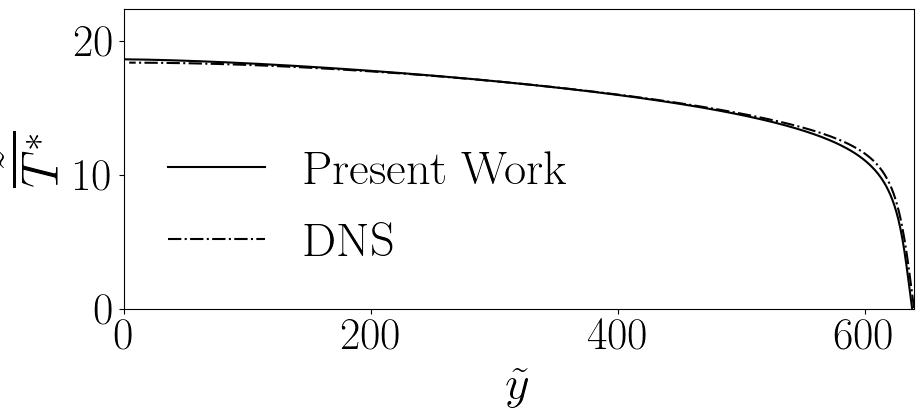
\includegraphics[angle=0, scale=0.34]{fotos_formatacao_final/Temperature_640_071_Prt(Ret)_A26}
		\subcaption{$Re_\tau = 640$, $L2_t = 0.17$}
	\end{minipage}
	\begin{minipage}[t]{0.45\textwidth}
		\centering
		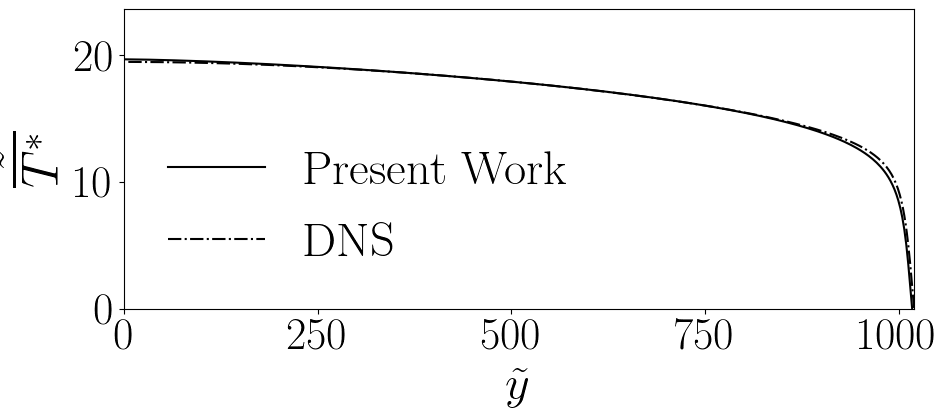
\includegraphics[angle=0, scale=0.34]{fotos_formatacao_final/Temperature_1000_071_Prt(Ret)_A26}
		\subcaption{$Re_\tau = 1020$, $L2_t = 0.14$}
	\end{minipage}	
	\caption{Resultados de temperatura para $Pr_\tau(Re_\tau)$, $A = 26$ e $Pr =0.71$. }
	\label{figura_9}
\end{figure*}

Outras formas de diminuir os erros foram buscadas. O perfil de velocidade era uma possibilidade, pois desempenha um papel importante no erro do método. Foram realizadas simulações desenvolvendo apenas esta propriedade física, e também houve erro associado (fig.\ref{figura_10}).

\begin{figure*}[!h]
	\centering
	\begin{minipage}[t]{0.5\textwidth}
		\centering
		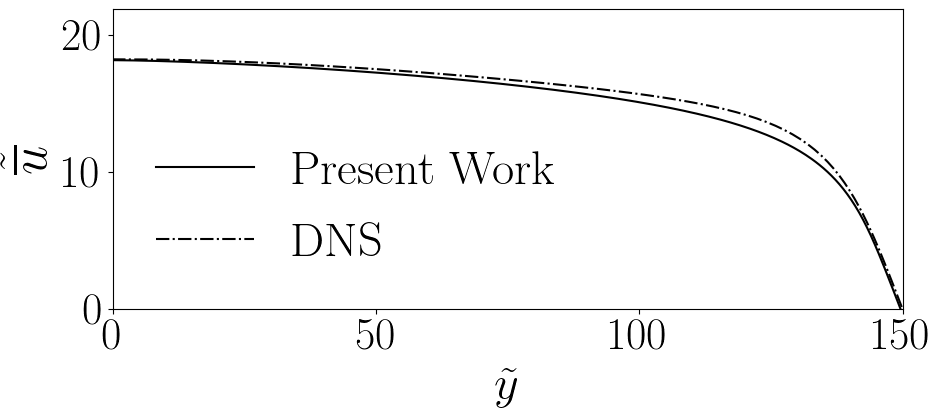
\includegraphics[angle=0, scale=0.34]{fotos_formatacao_final/Temperature_150_Avelocity}
		\subcaption{$Re_\tau = 150$, $L2_d = 0.47$}
	\end{minipage}
	\begin{minipage}[t]{0.45\textwidth}
		\centering
		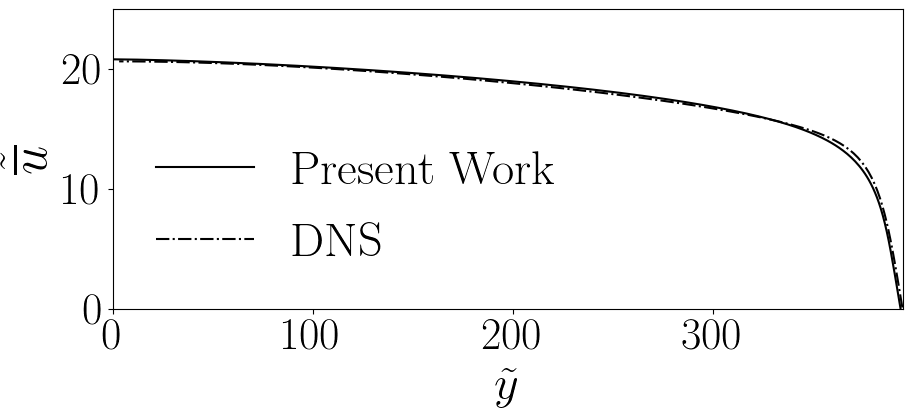
\includegraphics[angle=0, scale=0.34]{fotos_formatacao_final/Temperature_395_Avelocity}
		\subcaption{$Re_\tau = 395$, $L2_d = 0.17$}
	\end{minipage}
	\begin{minipage}[t]{0.5\textwidth}
		\centering
		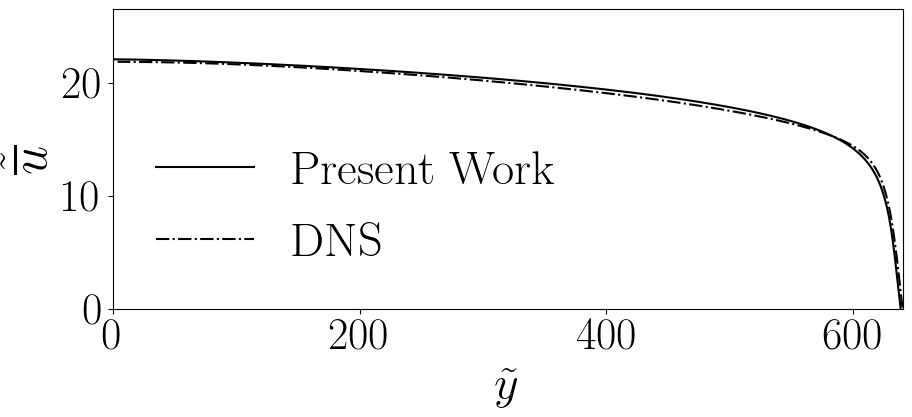
\includegraphics[angle=0, scale=0.34]{fotos_formatacao_final/Temperature_640_Avelocity}
		\subcaption{$Re_\tau = 640$, $L2_d = 0.23$}
	\end{minipage}
	\begin{minipage}[t]{0.45\textwidth}
		\centering
		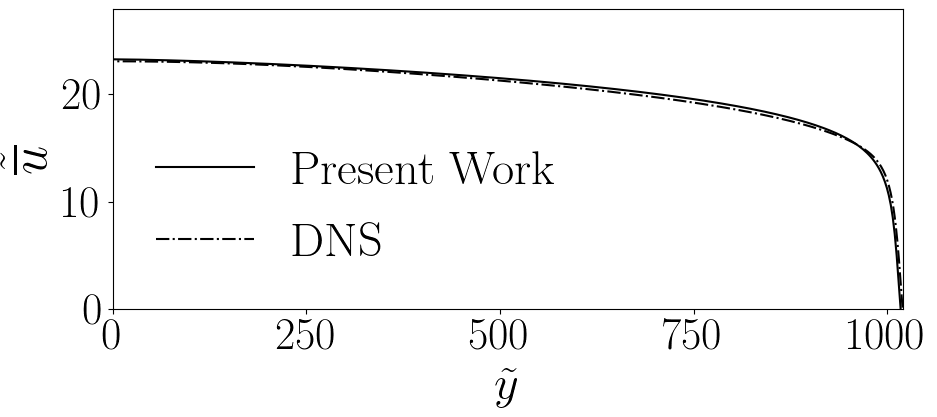
\includegraphics[angle=0, scale=0.34]{fotos_formatacao_final/Temperature_1000_Avelocity}
		\subcaption{$Re_\tau = 1020$, $L2_d = 0.23$}
	\end{minipage}	
	\caption{Resultados de perfil de velocidade para $A = 26$.}
	\label{figura_10}
\end{figure*}

Um modelo ajustado foi proposto no presente trabalho para a constante de cebeci, $A$, com o objetivo de redução no erro. O mesmo algorítmo usado para se achar o número de prandtl turbulento ideal foi utilizado para se encontrar a constante de Cebeci ideal. A velocidade do DNS foi utilizada para o cálculo do erro (norma L2).

Os resulados para a constante de Cebeci ideal são apresentados na tabela \ref{tablea}:

\begin{table}[!h]
	\centering
	\caption{Constante de Cebeci ideal ajustada para cada número de Reynolds turbulento.}
	\begin{tabular}{ll}
		\hline
		$Re_\tau$ & $A$\\
		\hline
		150  &   28.616180\\
		395  &   25.673782\\
		640  &   25.001266\\
		1020 &   25.002136\\ 
		\hline
	\end{tabular}
	\label{tablea}
\end{table}

Foi possível observar que para altos valores de Reynolds, a constante se aproximou no valor canônico encontrado na literatura, enquanto para baixos valores de número de Reynolds turbulento houve grande divergência.

Dessa forma, com os pontos encontrados e listados na tabela, foi possível realizar um encaixe de curva para se encontrar a função que fornece o número de Cebeci ideal a partir do número de Reynolds turbulento.

A partir destes resultados foi possível a criação de um modelo para a constante de Cebeci, que pode ser visto na equação que segue:

\begin{equation}\label{Amodelado}
A \left( Re_\tau\right)= \frac{Re_\tau ^{0.0451 * \ln(Re_\tau)} *e ^ {5.2753} }{Re_\tau ^{0.6094}}.
\end{equation}

Assim, a partir destes novos valores de Cebeci ajustados, foi possível o desenvolvimento de simulações de velocidade mais acuradas como se pode ver nos resultados que seguem:

\begin{figure*}[!h]
	\centering
	\begin{minipage}[t]{0.5\textwidth}
		\centering
		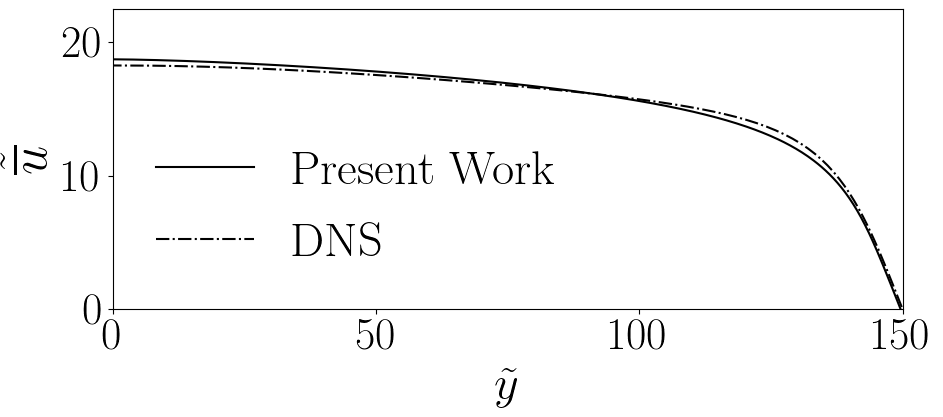
\includegraphics[angle=0, scale=0.34]{fotos_formatacao_final/Temperature_150_Amodeled}
		\subcaption{$Re_\tau = 150$, $L2_d = 0.28$}
	\end{minipage}
	\begin{minipage}[t]{0.45\textwidth}
		\centering
		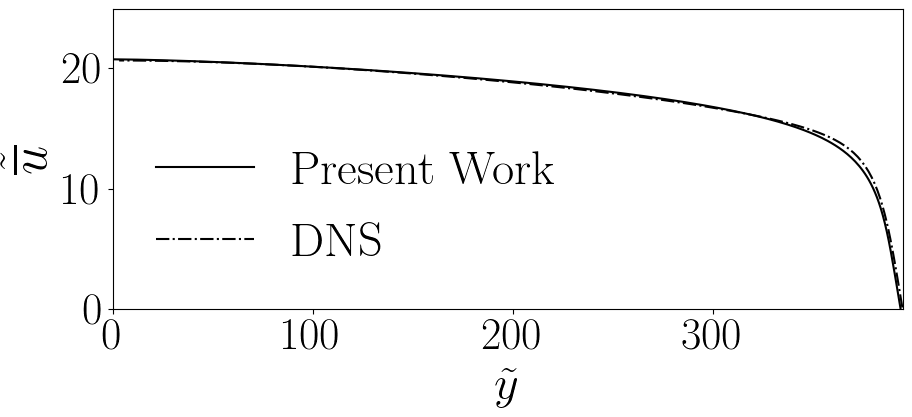
\includegraphics[angle=0, scale=0.34]{fotos_formatacao_final/Temperature_395_Amodeled}
		\subcaption{$Re_\tau = 395$, $L2_d = 0.16$}
	\end{minipage}
	\begin{minipage}[t]{0.5\textwidth}
		\centering
		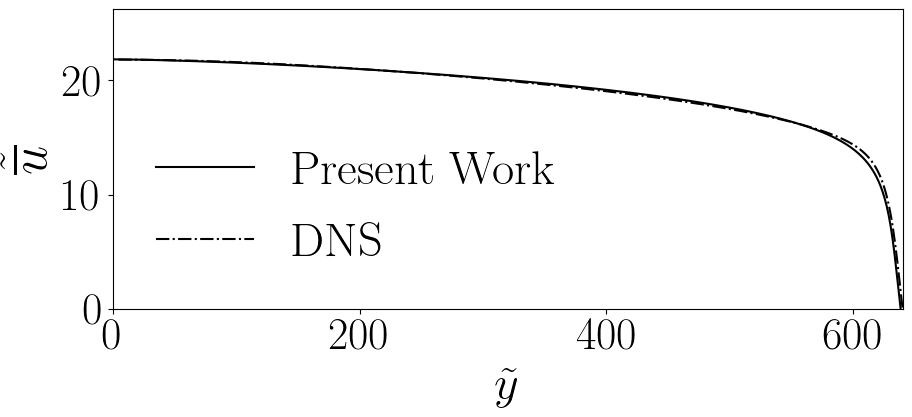
\includegraphics[angle=0, scale=0.34]{fotos_formatacao_final/Temperature_640_Amodeled}
		\subcaption{$Re_\tau = 640$, $L2_d = 0.14$}
	\end{minipage}
	\begin{minipage}[t]{0.45\textwidth}
		\centering
		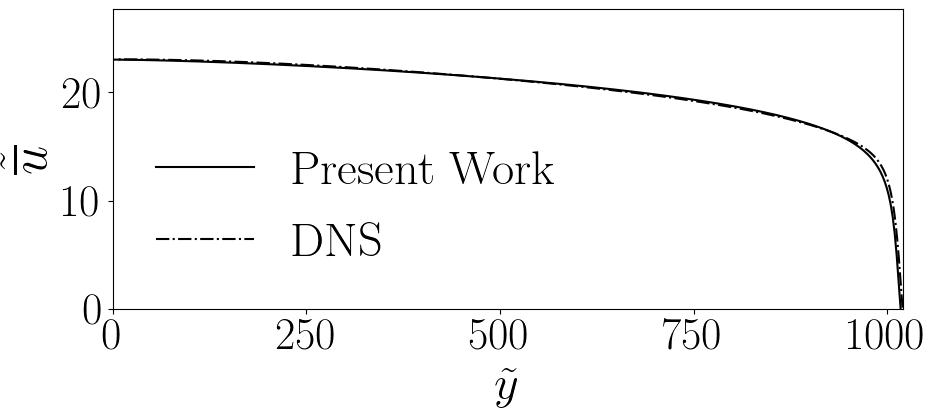
\includegraphics[angle=0, scale=0.34]{fotos_formatacao_final/Temperature_1000_Amodeled}
		\subcaption{$Re_\tau = 1020$, $L2_d = 0.13$}
	\end{minipage}	
	\caption{Resultados em distribuição de velocidade para o modelo de A \ref{Amodelado}.}
\end{figure*}

Com a função de Cebeci ajustada, um novo grupo de otimizações foi feito, com a mesma metodologia de evolução diferencial, levando em consideração esta nova formulação para a constante de cebeci. Tal estudo resultou em um novo conjunto de número de prandtl turbulento ótimo para cada número de 
Reynolds turbulento, como segue:

\begin{table}[!h]
	\centering
	\caption{Números de prandtl turbulentos ideais ajustados para cada número de Reynolds turbulento, com a função de Cebeci ajustada.}
	\begin{tabular}{ll}
		\hline
		$Re_\tau$ & $Pr_t$\\
		\hline
		150  &   0.88594\\
		395  &   0.90156\\
		640  &   0.91094\\
		1020 &   0.91406\\ 
		\hline
	\end{tabular}
\end{table}

Assim um novo modelo pode ser proposto para o número de Prandtl turbulento:

\begin{equation}
  \begin{split}
    Pr_t = 4.5290 * 10^{-12} Re_\tau^3 - 5.7395 * 10^{-8} Re_\tau^2 + 9.397 * 10^{-5} Re_\tau + 0.8731.
  \end{split}
\end{equation}

\vspace{0.5cm}

Esse novo modelo pode ser considerado mais acurado, uma vez que ele foi desenvolvido minimizando-se os erros advindos da simulação térmica.

Com esta nova parametrização, uma nova série de simulações foram desenvolvidas para se obter a temperatura no canal:
   
\begin{figure*}[!h]
	\centering
	\begin{minipage}[t]{0.5\textwidth}
		\centering
		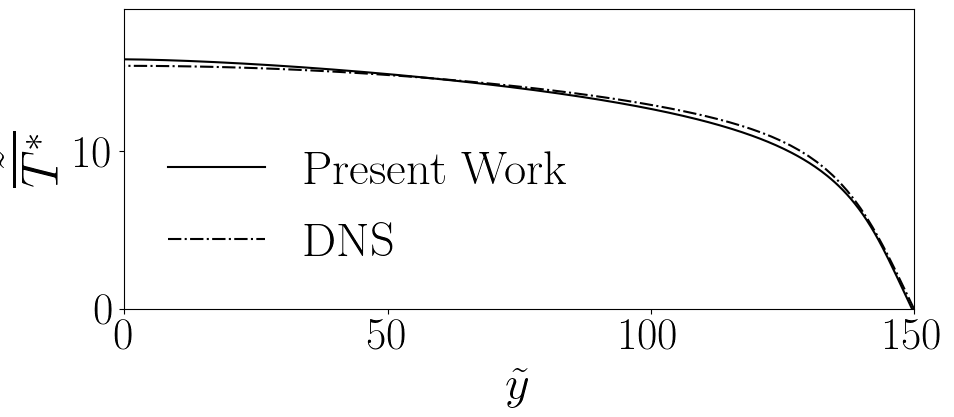
\includegraphics[angle=0, scale=0.34]{fotos_formatacao_final/Temperature_150_071_Prt(Ret)_Avelocity}
		\subcaption{$Re_\tau = 150$, $L2_t = 0.212$}
	\end{minipage}
	\begin{minipage}[t]{0.45\textwidth}
		\centering
		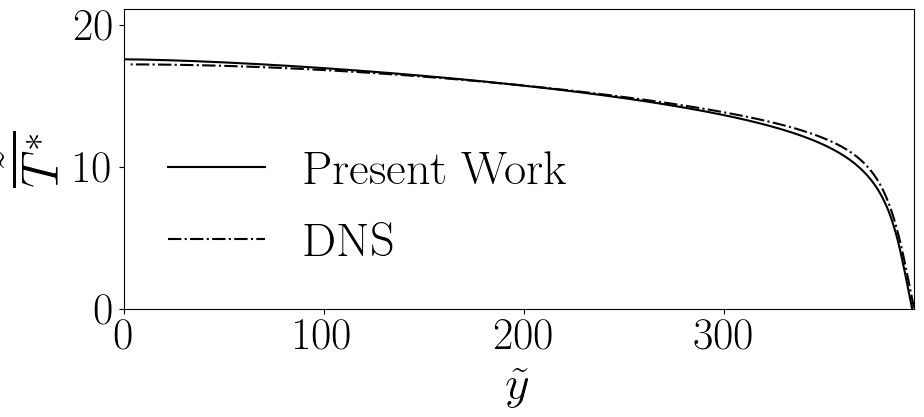
\includegraphics[angle=0, scale=0.34]{fotos_formatacao_final/Temperature_395_071_Prt(Ret)_Avelocity}
		\subcaption{$Re_\tau = 395$, $L2_t = 0.233$}
	\end{minipage}
	\begin{minipage}[t]{0.5\textwidth}
		\centering
		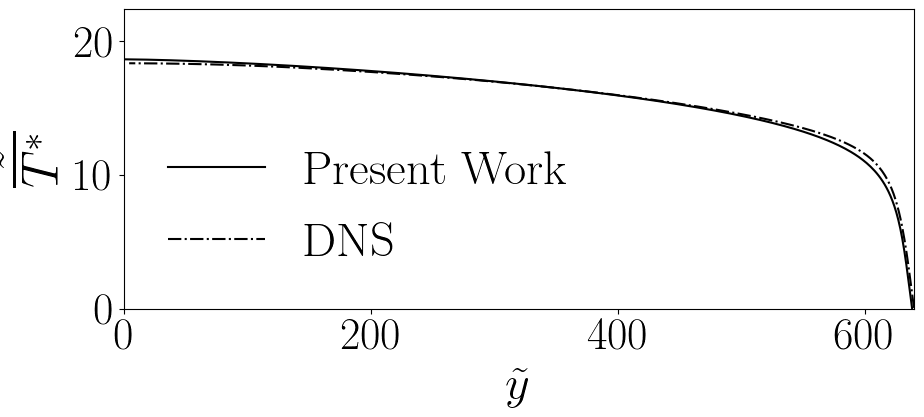
\includegraphics[angle=0, scale=0.34]{fotos_formatacao_final/Temperature_640_071_Prt(Ret)_Avelocity}
		\subcaption{$Re_\tau = 640$, $L2_t = 0.205$}
	\end{minipage}
	\begin{minipage}[t]{0.45\textwidth}
		\centering
		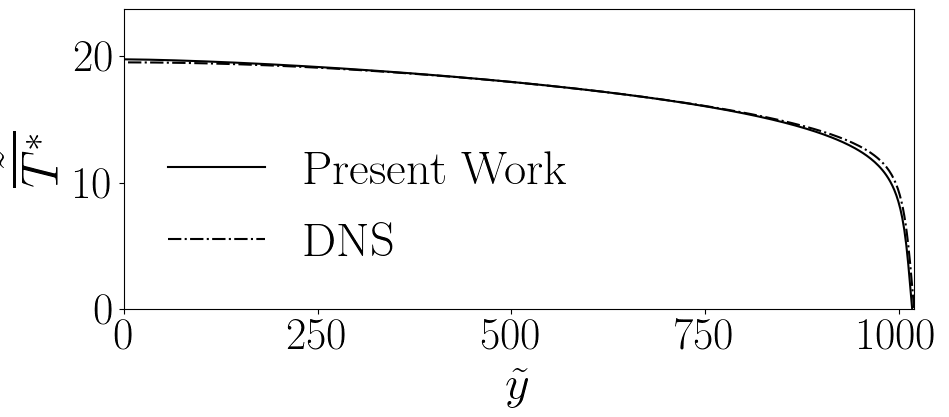
\includegraphics[angle=0, scale=0.34]{fotos_formatacao_final/Temperature_1000_071_Prt(Ret)_Avelocity}
		\subcaption{$Re_\tau = 1020$, $L2_t = 0.175$}
	\end{minipage}	
	\caption{Resultados térmicos para $Pr_\tau(Re\tau)$, $A(Re_\tau)$ e $Pr =0.71$ }
\end{figure*}

Os valores de Cebeci que resularam em um erro menor para a velocidade não tiveram o mesmo efeito na temperatura. Do ponto de vista algébrico, a constante de Cebeci aparece duas vezes: sob um contexto térmico e sob um contexto dinâmico (\ref{equationultima} e \ref{finalequationvelocity}).

Então, como última tentativa de melhorar o modelo, foi feita uma nova otimização, dessa vez, considerando a constante de Cebeci de forma separada no contexto da temperatura ($A_t$) e no contexto da velocidade ($A_d$).

Outro método de ajuste a partir de evolução diferencial é o ajuste multiobjetivo. Tal abordagem foi utilizada para considerar mais de uma variável para edição simultaneamente durante a otimização. Este método foi usado para ajustar a função térmica de cebeci e o número de Prandtl turbulento para o menor erro (norma L2) no campo de temperatura resultante para cada amostra DNS. A função cebeci para velocidade foi considerada no desenvolvimento anterior. Novos valores ideais foram encontrados para o número de Prandtl turbulento e a constante de cebeci térmica:

\begin{table}[!h]
	\centering
	\caption{Números de prandtl turbulentos ideais e função de cebeci térmica ($A_t$) ajustados para cada número de Reynolds turbulento, com a abordagem multiobjetiva.}
	\begin{tabular}{llll}
		\hline
		$Re_\tau$ & $Pr_t$ & $A_t$ & $A_d$\\
		\hline
		150  &   0.72530 & 37.25510 & 28.616180\\
		395  &   0.76821 & 34.24176 & 25.673782\\
		640  &   0.81896 & 31.27627 & 25.001266\\
		1020 &   0.86179 & 28.73726 & 25.002136\\ 
		\hline
	\end{tabular}
\end{table}

Com tais dados numéricos, novos modelos foram propostos para o número de prandtl turbulento e a função de cebeci termal:

\begin{equation}
  A_t = \frac{Re_\tau ^{0.0395 \ln(Re_\tau)^2 - 0.7588 \ln(Re_\tau) +  4.6637  } }{e ^{5.6703}},
\end{equation}

\begin{equation}
  \begin{split}
    Pr_t = -2.4892 * 10^{-10} Re_\tau^3 +  3.6036 * 10^{-7} Re_\tau^2 + 3.7921 *10 ^{-5} Re_\tau + 0.7123 .
  \end{split}
\end{equation}

Novas simulações foram feitas usando os novos modelos propostos:

\begin{figure*}[!h]
	\centering
	\begin{minipage}[t]{0.5\textwidth}
		\centering
		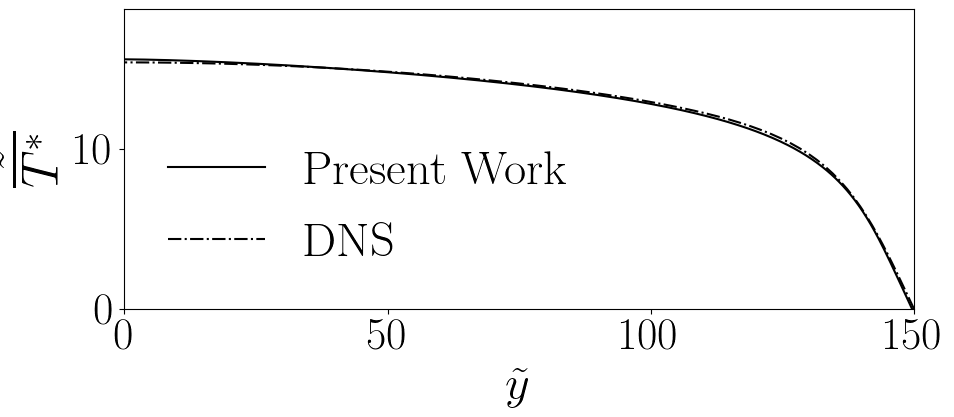
\includegraphics[angle=0, scale=0.24]{fotos_formatacao_final/Temperature_150_071_Genetic2temperature}
		\subcaption{$Re_\tau = 150$, $L2_t = 0.091$}
	\end{minipage}
	\begin{minipage}[t]{0.45\textwidth}
		\centering
		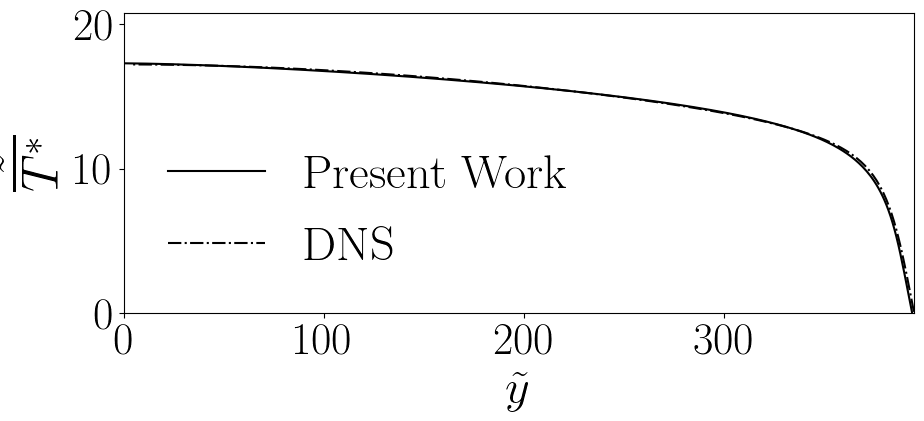
\includegraphics[angle=0, scale=0.24]{fotos_formatacao_final/Temperature_395_071_Genetic2temperature}
		\subcaption{$Re_\tau = 395$, $L2_t = 0.049$}
	\end{minipage}
	\begin{minipage}[t]{0.5\textwidth}
		\centering
		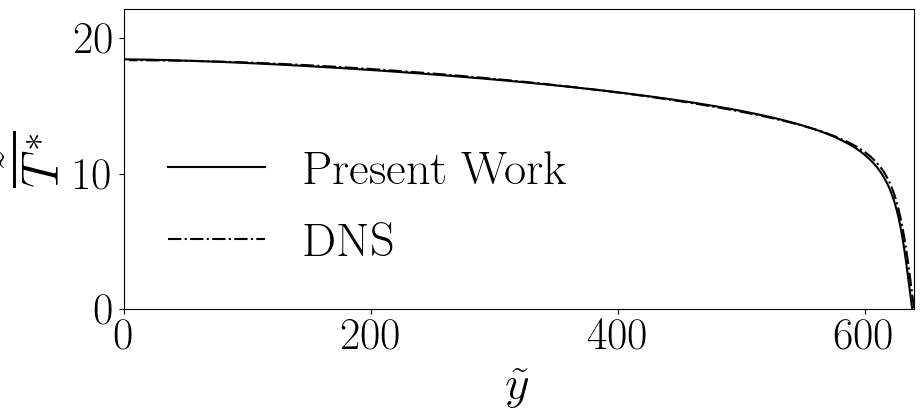
\includegraphics[angle=0, scale=0.24]{fotos_formatacao_final/Temperature_640_071_Genetic2temperature}
		\subcaption{$Re_\tau = 640$, $L2_t = 0.061$}
	\end{minipage}
	\begin{minipage}[t]{0.45\textwidth}
		\centering
		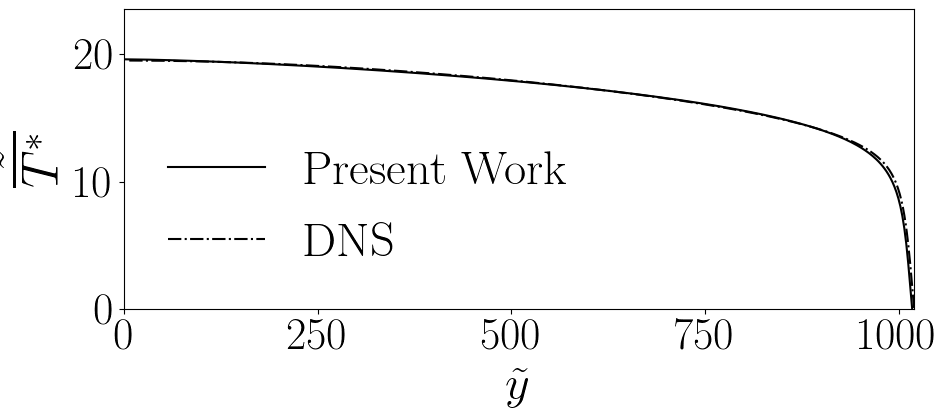
\includegraphics[angle=0, scale=0.24]{fotos_formatacao_final/Temperature_1000_071_Genetic2temperature}
		\subcaption{$Re_\tau = 1020$, $L2_t = 0.076$}
	\end{minipage}	
	\caption{Results of temperature simulations for $Pr_\tau(Re_\tau)$, $A_d(Re_\tau)$, $A_t(Re_\tau) $ and $Pr =0.71$, with multi-objective adjustment.}
\end{figure*}

Estes foram os melhores resultados obtidos.


\chapter{Simulações no MFsim}

Tendo-se estes novo modelos sido propostos, novas simulações foram feitas no MFsim, visando validar se estes modelos para a constante de Cebeci e o número de Prandtl turbulento tem utilidade em softwares comerciais de simulação fluidodinâmica.

\section{Sobre a parametrização do sistema}
Estabeleceu-se o domínio computacional como um paralelepípedo de dimensões $0.25m$ por $0.25m$ por $2m$, onde a dimensão maior seria a no sentido da corrente. A partir disso, calculou-se o gradiente de pressão a partir das seguintes equações:

\begin{equation}
  Re_\tau = \frac{u_\tau R}{\nu}
\end{equation}

\begin{equation}
  u_\tau = \sqrt{\frac{|\tau_w|}{\rho}}
\end{equation}

\begin{equation}
  \tau_w = \Delta P \frac{R}{L}
\end{equation}

Desenvolvimendo as equações acima, tem-se:

\begin{equation}
  \Delta P = \tau_w \frac{L}{R}
\end{equation}

\begin{equation}
  \tau_w = \rho u_\tau^2
\end{equation}

\begin{equation}
  u_\tau = \frac{\nu Re_\tau}{R}
\end{equation}


Assim, esbosa-se uma relação entre a diferença de pressão e o número de Reynolds:

\begin{equation}
  \Delta P = Re_\tau^2 \frac{L \mu^2}{\rho R^3}
\end{equation}

\begin{equation}
  \Delta P =3 Re \frac{L \mu^2}{\rho R^2}
\end{equation}

Adotam-se os seguintes valores:
\begin{itemize}
  \item $L = 2m$
  \item $R = 0.125m$
  \item $\mu = 0.1 kg/m.s$
  \item $\rho = 100 kg/m^3$
\end{itemize}

A partir destas equações é possível se calcular o valor da diferença de pressão entre a entrada e saída do fluxo a partir do número de Raynolds avaliado, segue uma tabela com os valores de diferença de pressão resultantes:

\begin{table}[!h]
  \centering
  \caption{Valores de diferença de pressão para cada número de Reynolds turbulento.}
  \begin{tabular}{ll}
    \hline
    $Re_\tau$ & $\Delta P$ \\
    \hline
    150  &   2304 &
    395  &   15976,96 &
    640  &   41943,04 &
    1020 &   106536,96 &
    \hline
  \end{tabular}
\end{table}

\section{O domínio computacional}
Assim, para representar o domínio, uma malha de $200$ volumes por $25$ volumes por $25$ volumes. O que resultou em volumes cúbicos de $0.01cm$ de tamanho. A malha gerada pode ser vista na figura \ref{fig:malha}:

\begin{figure}[!h]
  \centering
  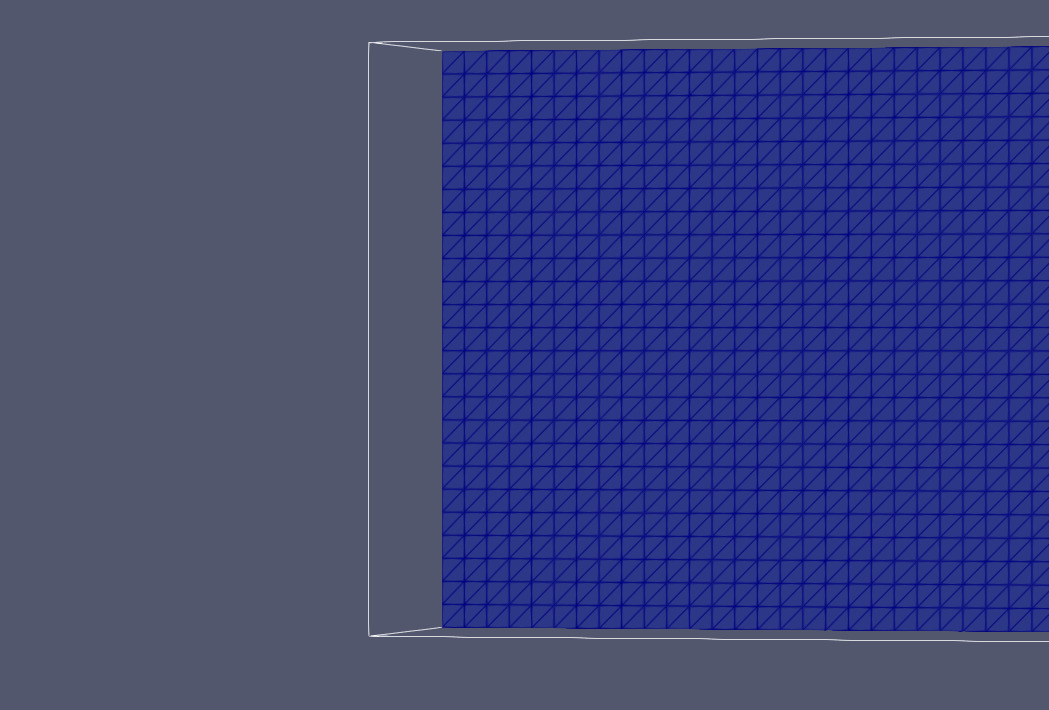
\includegraphics[angle=0, scale=0.25]{cap_fundamentacao/domain_mesh.jpeg}
  \caption{Malha gerada para a simulação.}
  \label{fig:malha}
\end{figure}

Para a condição de contorno estipulou-se dirichlet para a presão nas paredes perpendiculares ao eixo $x$ (no sentido da corrente), a partir dos valores caluclados anteriormente, assim como nas paredes perpendiculares ao eixo $z$, enquanto as velocidades foram mantidas como newmann, considerando-se auto similaridade no eixo $z$. Já nas paredes perpendiculares ao eixo $y$, configuraram-se as velocidades iqual a zero, uma vez que é onde estão localizadas as paredes em condição de não escorregamento. Os resultados iniciais podem ser vistos adiante (\ref{fig:first_results}):

\begin{figure}[!h]
  \centering
  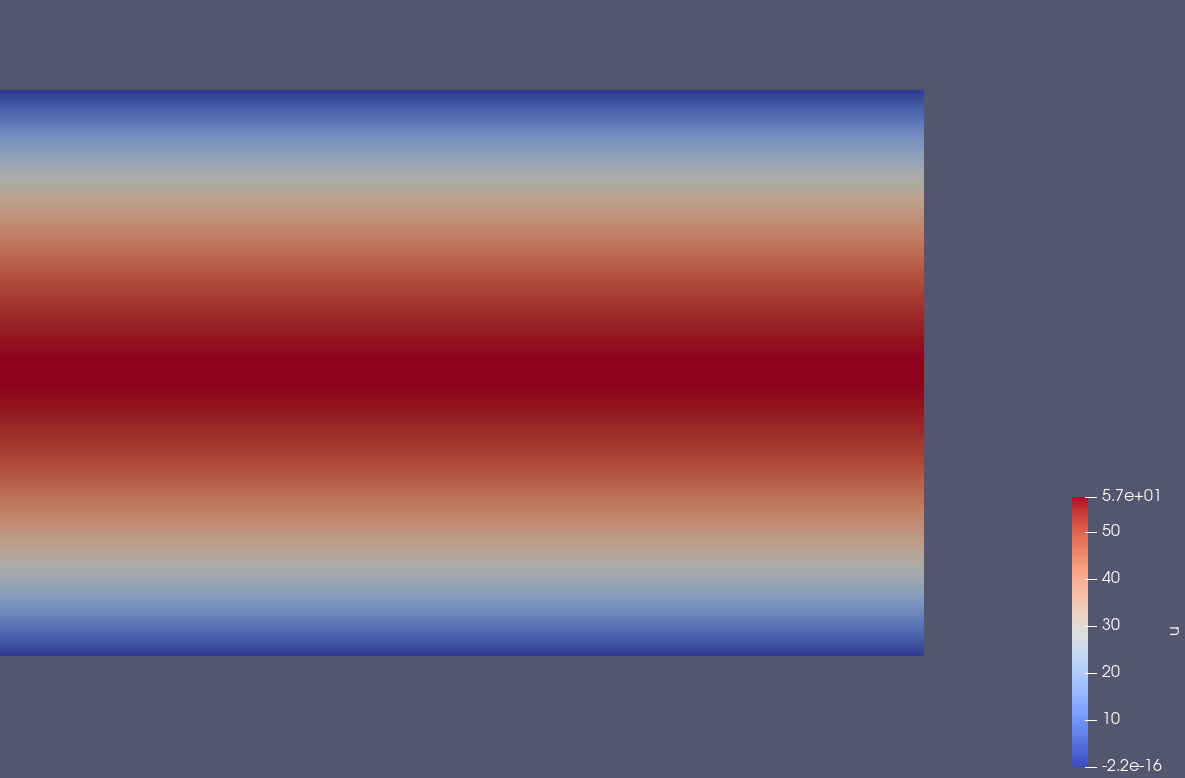
\includegraphics[angle=0, scale=0.25]{cap_fundamentacao/first_results.png}
  \caption{Resultados para $Re_\tau = 150$.}
  \label{fig:first_results}
\end{figure}

Notou-se que a velocidade no meio do canal ficou próximo de $57 m/s$, que ao adimensionalizar ($\tilde{u} = \frac{u}{u_\tau}$ e $u_\tau = \frac{\mu Re_\tau}{\rho R}$) é igual a 47.5, que é bem distante do valor de velocidade calculado para os mesmos valores de constante de cebeci e número de prandtl turbulento, que deveria ser por volta de 18 m/s. Por se distanciar do DNS também, pode ser algo errado com a determinação do Reynolds turbulento.


% ----------------------------------------------------------
% Proposta de pesquisa
% ----------------------------------------------------------
% \chapter[Ensaios numéricos]{Ensaios numéricos}

\section{Caso da esfera}
\section{Caso do canal de Poiseuille}
\section{Caso da cavidade com tampa deslizante}
\section{Caso da cavidade com convecção natural}

% ---
% Finaliza a parte no bookmark do PDF, para que se inicie o bookmark na raiz
% ---
% \bookmarksetup{startatroot}% 
% ---

% ---
% Conclusão
% ---
\chapter[Conclusão]{Conclusão}

No presente trabalho, os autores desenvolveram de forma bem sucedida um métod semi-analítico para o cálculo do campo de temperatura sobre um escoamento turbulento em canal de Poiseuille, validando-se os resultados com os de DNS. Durante o estudo, observou-se a influência que os parâmetros da constante de Cebeci e o número de Prandtl turbulento tinham sobre os resultados, e constatou-se que o valor canônico do Prandtl turbulento de $0.7$, que fora usado nas simulações não correspondia aos observados nas simulações de DNS, que variavam não só com o número de Reynolds turbulento, mas também com a distância da parede.

A partir dessas observações, novos modelos foram criados para descrever essa grandeza de forma que tornou-se os resultados do presente estudo mais representativos. Tais modelos ajustados foram criados a partir de métodos de evolução diferencial, que otimizaram o sistema para a menor norma L2 quando comparado com a solução numérica em DNS.

Os resultados obtidos com o modelo ajustado foram satisfatórios, e mostraram-se mais próximos dos resultados em DNS que a simulação desenvolvida usando-se o número de Prandtl turbulento advindo da própria solução DNS, o que mostra que o método de otimização ajustou o sistema de forma a corrigir distorções advindas não só do Prandtl turbulento, mas também de outros ajustes feitos durante o desenvolvimento do método semi-analítico.



 

% ----------------------------------------------------------
% ELEMENTOS PÓS-TEXTUAIS
% ----------------------------------------------------------
% \postextual

% ----------------------------------------------------------
% Referências bibliográficas
% ----------------------------------------------------------
\bibliography{bib/abntex2-modelo-references}

% ----------------------------------------------------------
% Glossário
% ----------------------------------------------------------
%
%\glossary

% ----------------------------------------------------------
% Apêndices
% ----------------------------------------------------------
% ---
% Inicia os apêndices
% ---
%\begin{apendicesenv}
% Imprime uma página indicando o início dos apêndices
%\partapendices
% ----------------------------------------------------------
% Incluir Apêndice
% ----------------------------------------------------------
% ----------------------------------------------------------
% Capitulo com exemplos de comandos inseridos de arquivo externo 
% ----------------------------------------------------------
%%% abtex2-modelo-include-comandos.tex, v-1.4 laurocesar
%% Copyright 2012-2013 by abnTeX2 group at http://abntex2.googlecode.com/ 
%%
%% This work may be distributed and/or modified under the
%% conditions of the LaTeX Project Public License, either version 1.3
%% of this license or (at your option) any later version.
%% The latest version of this license is in
%%   http://www.latex-project.org/lppl.txt
%% and version 1.3 or later is part of all distributions of LaTeX
%% version 2005/12/01 or later.
%%
%% This work has the LPPL maintenance status `maintained'.
%% 
%% The Current Maintainer of this work is the abnTeX2 team, led
%% by Lauro César Araujo. Further information are available on 
%% http://abntex2.googlecode.com/
%%
%% This work consists of the files abntex2-modelo-include-comandos.tex
%%

% ---
% Este capítulo, utilizado por diferentes exemplos do abnTeX2, ilustra o uso de
% comandos do abnTeX2 e de LaTeX.
% ---
 
\chapter{Resultados de comandos}\label{cap_exemplos}

\chapterprecishere{Isto é uma sinopse de capítulo. A ABNT não traz nenhuma
normatização a respeito desse tipo de resumo, que é mais comum em romances 
e livros técnicos.}\index{sinopse de capítulo}

% ---
\section{Citações}
% ---

\index{citações!diretas}Utilize o ambiente \texttt{citacao} para incluir
citações diretas com mais de três linhas:

\begin{citacao}
As citações diretas, no texto, com mais de três linhas, devem ser
destacadas com recuo de 4 cm da margem esquerda, com letra menor que a do texto
utilizado e sem as aspas. No caso de documentos datilografados, deve-se
observar apenas o recuo \cite[5.3]{NBR10520:2002}.
\end{citacao}

\index{citações!simples}Citações simples, com até três linhas, devem ser
incluídas com aspas. Observe que em \LaTeX~ as aspas iniciais são diferentes das finais: ``Amor é fogo que
arde sem se ver''. 


% ---
\section{Remissões internas}
% ---

Ao nomear a \autoref{tab-nivinv}, apresentamos um exemplo de remissão interna,
que também pode ser feita quando indicamos o \autoref{cap_exemplos}\footnote{O
número do capítulo indicado é
\ref{cap_exemplos}, que se inicia à página \pageref{cap_exemplos}.}
(\nameref{cap_exemplos}, \autopageref{cap_exemplos}), por exemplo.

% ---
\section{Tabelas}
% ---

Apresenta-se um exemplo de tabela a ser confeccionada. Atente-se para as normas de tabela exigidas pela Universidade.

\index{tabelas}A \autoref{tab-nivinv} é um exemplo de tabela construída em
\LaTeX.

\begin{table}[htb]
\footnotesize
\caption[Níveis de investigação]{Níveis de investigação.}
\label{tab-nivinv}
\begin{tabular}{p{2.6cm}|p{6.0cm}|p{2.25cm}|p{3.40cm}}
  %\hline
   \textbf{Nível de Investigação} & \textbf{Insumos}  & \textbf{Sistemas de Investigação}  & \textbf{Produtos}  \\
    \hline
    Meta-nível & Filosofia\index{filosofia} da Ciência  & Epistemologia &
    Paradigma  \\
    \hline
    Nível do objeto & Paradigmas do metanível e evidências do nível inferior &
    Ciência  & Teorias e modelos \\
    \hline
    Nível inferior & Modelos e métodos do nível do objeto e problemas do nível inferior & Prática & Solução de problemas  \\
   % \hline
\end{tabular}
\legend{Fonte: \citeonline{van86}}
\end{table}


\section{Figuras}

\index{figuras}Figuras podem ser criadas diretamente em \LaTeX,
como o exemplo da \autoref{fig_circulo}.

\begin{figure}[htb]
	\begin{center}
	    \setlength{\unitlength}{5cm}
		\begin{picture}(1,1)
		\put(0,0){\line(0,1){1}}
		\put(0,0){\line(1,0){1}}
		\put(0,0){\line(1,1){1}}
		\put(0,0){\line(1,2){.5}}
		\put(0,0){\line(1,3){.3333}}
		\put(0,0){\line(1,4){.25}}
		\put(0,0){\line(1,5){.2}}
		\put(0,0){\line(1,6){.1667}}
		\put(0,0){\line(2,1){1}}
		\put(0,0){\line(2,3){.6667}}
		\put(0,0){\line(2,5){.4}}
		\put(0,0){\line(3,1){1}}
		\put(0,0){\line(3,2){1}}
		\put(0,0){\line(3,4){.75}}
		\put(0,0){\line(3,5){.6}}
		\put(0,0){\line(4,1){1}}
		\put(0,0){\line(4,3){1}}
		\put(0,0){\line(4,5){.8}}
		\put(0,0){\line(5,1){1}}
		\put(0,0){\line(5,2){1}}
		\put(0,0){\line(5,3){1}}
		\put(0,0){\line(5,4){1}}
		\put(0,0){\line(5,6){.8333}}
		\put(0,0){\line(6,1){1}}
		\put(0,0){\line(6,5){1}}
		\end{picture}
	\end{center}
	\caption{\label{fig_circulo}A delimitação do espaço}
	\legend{Fonte: os autores}
\end{figure}

Ou então figuras podem ser incorporadas de arquivos externos, como é o caso da
\autoref{fig_grafico}. Se a figura que ser incluída se tratar de um diagrama, um
gráfico ou uma ilustração que você mesmo produza, priorize o uso de imagens
vetoriais no formato PDF. Com isso, o tamanho do arquivo final do trabalho será
menor, e as imagens terão uma apresentação melhor, principalmente quando
impressas, uma vez que imagens vetorias são perfeitamente escaláveis para
qualquer dimensão. Nesse caso, se for utilizar o Microsoft Excel para produzir
gráficos, ou o Microsoft Word para produzir ilustrações, exporte-os como PDF e
os incorpore ao documento conforme o exemplo abaixo. No entanto, para manter a
coerência no uso de software livre (já que você está usando \LaTeX e \abnTeX),
teste a ferramenta \textsf{InkScape}\index{InkScape}
(\url{http://inkscape.org/}). Ela é uma excelente opção de código-livre para
produzir ilustrações vetoriais, similar ao CorelDraw\index{CorelDraw} ou ao Adobe
Illustrator\index{Adobe Illustrator}. De todo modo, caso não seja possível
utilizar arquivos de imagens como PDF, utilize qualquer outro formato, como
JPEG, GIF, BMP, etc. Nesse caso, você pode tentar aprimorar as imagens
incorporadas com o software livre \textsf{Gimp}\index{Gimp}
(\url{http://www.gimp.org/}). Ele é uma alternativa livre ao Adobe
Photoshop\index{Adobe Photoshop}.

\begin{figure}[htb]
	\begin{center}
	    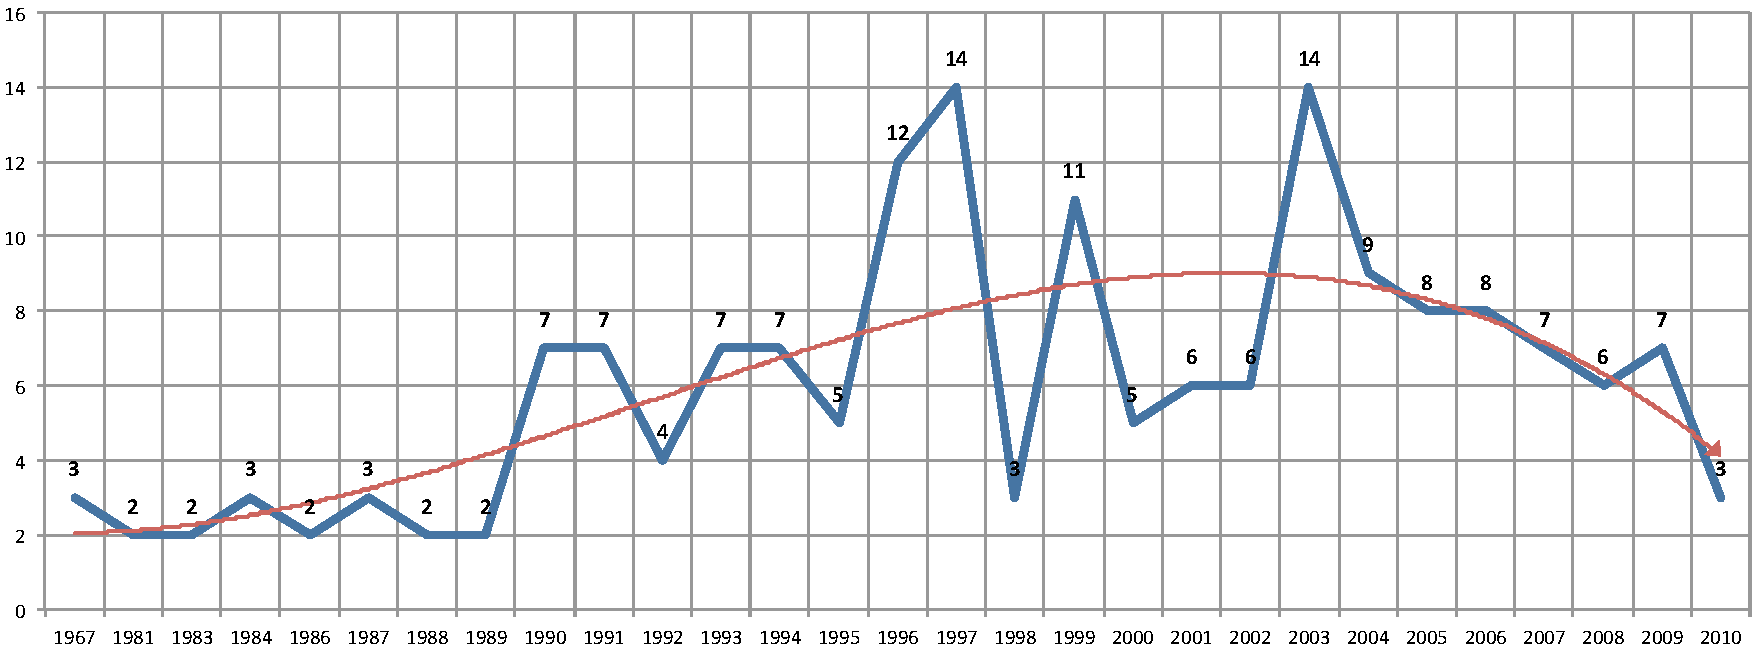
\includegraphics[scale=0.5]{ape_comandos/abntex2-modelo-img-grafico.pdf}
	\end{center}
	\caption{\label{fig_grafico}Gráfico produzido em Excel e salvo como PDF}
	\legend{Fonte: \citeonline[p. 24]{araujo2012}}
\end{figure}

% ---
\section{Enumerações: alíneas e subalíneas}
% ---

\index{alíneas}\index{subalíneas}\index{incisos}Quando for necessário enumerar
os diversos assuntos de uma seção que não possua título, esta deve ser
subdividida em alíneas \cite[4.2]{NBR6024:2012}:

\begin{alineas}

  \item os diversos assuntos que não possuam título próprio, dentro de uma mesma
  seção, devem ser subdivididos em alíneas\footnote{As notas devem ser digitadas ou datilografadas
  dentro das margens, ficando separadas do texto por um espaço simples de entre as
  linhas e por filete de 5 cm, a partir da margem esquerda. Devem ser
  alinhadas, a partir da segunda linha da mesma nota, abaixo da primeira letra
  da primeira palavra, de forma a destacar o expoente, sem espaço entre elas e
  com fonte menor. \citeonline[5.2.1]{NBR14724:2011}}; 
  
  \item o texto que antecede as alíneas termina em dois pontos;
  \item as alíneas devem ser indicadas alfabeticamente, em letra minúscula,
  seguida de parêntese. Utilizam-se letras dobradas, quando esgotadas as
  letras do alfabeto;

  \item as letras indicativas das alíneas devem apresentar recuo em relação à
  margem esquerda;

  \item o texto da alínea deve começar por letra minúscula e terminar em
  ponto-e-vírgula, exceto a última alínea que termina em ponto final;

  \item o texto da alínea deve terminar em dois pontos, se houver subalínea;

  \item a segunda e as seguintes linhas do texto da alínea começa sob a
  primeira letra do texto da própria alínea;
  
  \item subalíneas \cite[4.3]{NBR6024:2012} devem ser conforme as alíneas a
  seguir:

  \begin{alineas}
     \item as subalíneas devem começar por travessão seguido de espaço;

     \item as subalíneas devem apresentar recuo em relação à alínea;

     \item o texto da subalínea deve começar por letra minúscula e terminar em
     ponto-e-vírgula. A última subalínea deve terminar em ponto final, se não
     houver alínea subsequente;

     \item a segunda e as seguintes linhas do texto da subalínea começam sob a
     primeira letra do texto da própria subalínea.
  \end{alineas}
  
  \item no \abnTeX\ estão disponíveis os ambientes \texttt{incisos} e
  \texttt{subalineas}, que em suma são o mesmo que se criar outro nível de
  \texttt{alineas}, como nos exemplos à seguir:
  
  \begin{incisos}
    \item \textit{Um novo inciso em itálico};
  \end{incisos}
  
  \item Alínea em \textbf{negrito}:
  
  \begin{subalineas}
    \item \textit{Uma subalínea em itálico};
    \item \underline{\textit{Uma subalínea em itálico e sublinhado}}; 
  \end{subalineas}
  
  \item Última alínea com \emph{ênfase}.
  
\end{alineas}


% ---
\section{Inclução de outros arquivos}\label{sec-include}
% ---

É uma boa prática dividir o seu documento em diversos arquivos, e não
apenas escrever tudo em um único. Esse recurso foi utilizado neste
documento. Para incluir diferentes arquivos em um arquivo principal,
de modo que cada arquivo incluído fique em uma página diferente, utilize o
comando:

\begin{verbatim}
   \include{documento-a-ser-incluido}      % sem a extensão .tex
\end{verbatim}

Para incluir documentos sem quebra de páginas, utilize:

\begin{verbatim}
   \input{documento-a-ser-incluido}      % sem a extensão .tex
\end{verbatim}

% ---
\section{Compilar o documento \LaTeX}
% ---

Geralmente os editores \LaTeX, como o
TeXlipse\footnote{\url{http://texlipse.sourceforge.net/}}, o
Texmaker\footnote{\url{http://www.xm1math.net/texmaker/}}, entre outros,
compilam os documentos automaticamente, de modo que você não precisa se
preocupar com isso.

No entanto, você pode compilar os documentos \LaTeX usando os seguintes
comandos, que devem ser digitados no \emph{Prompt de Comandos} do Windows ou no
\emph{Terminal} do Mac ou do Linux:

\begin{verbatim}
   pdflatex ARQUIVO_PRINCIPAL.tex
   bibtex ARQUIVO_PRINCIPAL.aux
   makeindex ARQUIVO_PRINCIPAL.idx 
   makeindex ARQUIVO_PRINCIPAL.nlo -s nomencl.ist -o ARQUIVO_PRINCIPAL.nls
   pdflatex ARQUIVO_PRINCIPAL.tex
   pdflatex ARQUIVO_PRINCIPAL.tex
\end{verbatim}

% ---
\section{Divisões do documento: seção}\label{sec-divisoes}
% ---

Esta seção testa o uso de divisões de documentos. Isto é uma seção.

\subsection{Divisões do documento: subseção}

Isto é uma subseção.

\subsubsection{Divisões do documento: subsubseção}

Isto é uma subsubseção.

\subsubsection{Divisões do documento: subsubseção}

Isto é outra subsubseção.

\subsection{Divisões do documento: subseção}\label{sec-exemplo-subsec}

Isto é uma subseção.

\subsubsection{Divisões do documento: subsubseção}

Isto é mais uma subsubseção da \autoref{sec-exemplo-subsec}.

% ---
\section{Este é um exemplo de nome de seção longo. Ele deve estar
alinhado à esquerda e a segunda e demais linhas devem iniciar logo abaixo da
primeira palavra da primeira linha}
% ---

Isso atende à norma \citeonline[seções de 5.2.2 a 5.2.4]{NBR14724:2011} 
 e \citeonline[seções de 3.1 a 3.8]{NBR6024:2012}.


% ---
\section{Consulte o manual da classe \textsf{abntex2}}
% ---

Consulte o manual da classe \textsf{abntex2} \cite{abntex2classe} para uma
referência completa das macros e ambientes disponíveis. Além disso, o manual
possui informações adicionais sobre as normas ABNT observadas pelo \abnTeX.

%\end{apendicesenv}
% ---

% ----------------------------------------------------------
% Anexos
% ----------------------------------------------------------
% ---
% Inicia os anexos
% ---
%\begin{anexosenv}
% Imprime uma página indicando o início dos anexos
%\partanexos
% ---
% Incluir Anexo
% ---
%\chapter{Manual de utilização do MFGui.}
%\label{anexo1}
%\lipsum[1-25]


%\end{anexosenv}


\end{document}
